%\PassOptionsToPackage{draft}{graphicx} % to leave out images and speed up compiler

\documentclass[xcolor=svgnames]{beamer}
%\documentclass[xcolor=svgnames]{beamer}
%\includeonlyframes{current}

\usepackage[utf8]    {inputenc}
\usepackage[T1]      {fontenc}
\usepackage[english] {babel}
\usepackage{fourier}

\usepackage{amsmath,amsfonts,graphicx}
\usepackage{beamerleanprogress}
\usepackage{xcolor}
\usepackage{soul}
\usepackage{multicol}
\usepackage{tikz} 
\usepackage[export]{adjustbox}

\definecolor{iyellow}{RGB}{255, 162, 23}
\definecolor{sgreen}{RGB}{118, 191, 138}

\usepackage{multicol}

\usepackage{upquote} % to convert funny quotes to straight quotes

\setbeamertemplate{theorems}[numbered] 



\newcommand{\yellow}[1]{\textcolor{iyellow}{#1}}
\newcommand{\green}[1]{\textcolor{sgreen}{#1}}
\newcommand{\red}[1]{\textcolor{red}{#1}}
\newcommand{\blue}[1]{{\textcolor{blue}{#1}}}
\newcommand{\answer}[1]{\textit{\textbf{\textcolor{iyellow}{#1}}}}

\newcommand{\cell}[1]{{\sf \textbf{\textcolor{DarkMagenta}{#1}}}}
\newcommand{\ra}{$\rightarrow$ }
\usetikzlibrary{shadows}

\newcommand*\keystroke[1]{%
  \tikz[baseline=(key.base)]
    \node[%
      draw,
      fill=white,
      drop shadow={shadow xshift=0.25ex,shadow yshift=-0.25ex,fill=black,opacity=0.75},
      rectangle,
      rounded corners=2pt,
      inner sep=1pt,
      line width=0.5pt,
      font=\scriptsize\sffamily
    ](key) {#1\strut}
  ;
}


\usepackage{hyperref}
\hypersetup{
    colorlinks=true,
    linkcolor=blue,
    filecolor=magenta,      
    urlcolor=cyan,
}
\usepackage{url}

\newcommand{\ukey}{\keystroke{Cmnd}/\keystroke{Ctrl}}



\title
  [Data 301 Data Analytics\hspace{2em}]
  {Data 301 Data Analytics\\
  Spreadsheets: Microsoft Excel\\
  Part 1 of 3}

\author
  [Dr.\ Irene Vrbik]
  {Dr.\ Irene Vrbik}

\date
  {}

\institute
  {University of British Columbia Okanagan \newline irene.vrbik@ubc.ca}



\begin{document}


\graphicspath{{img/}}


\maketitle



\section
  {Spreadsheets: Microsoft Excel}



\begin{frame}
  {Why Spreadsheets and Microsoft Excel?}
\emph{}Spreadsheets are the most common, general-purpose software for data analysis and reporting.\par \vspace{5mm} 
Microsoft Excel is the most popular spreadsheet program with hundreds of millions of installations. 
  \begin{itemize}
\item The spreadsheet concepts translate to other products.\\[4mm]
\end{itemize}
Excel and spreadsheets are not always the best tool for data analysis, but they are great for quick analysis, reporting, and sharing.\\
\medskip
Follow along with the examples by  downloading the {\bf 03ExcelPartI.xlsx} and {\bf DemoPartI.xlsx} file from CANVAS.
\end{frame}

\begin{frame}{Spreadsheet Overview}
A spreadsheet organizes information into a two-dimensional array of cells (a table).\par \vspace{5mm} 
A cell has two components: 
\begin{itemize}
\item an address - specified given a column letter and row number 
\item a location - that can store a number, text, or formula \\[4mm]
\end{itemize}
The power of a spreadsheet is that we can write simple formulas (commands) to perform calculations and immediately see the results of those calculations.\par \vspace{5mm} 
Spreadsheets are very common in business and reporting applications.
\end{frame}

%
%\begin{frame}{Try it!}
%Follow along with these examples by  downloading the {\bf 03ExcelPartI.xlsx} and {\bf DemoPartI.xlsx} file from CANVAS.
%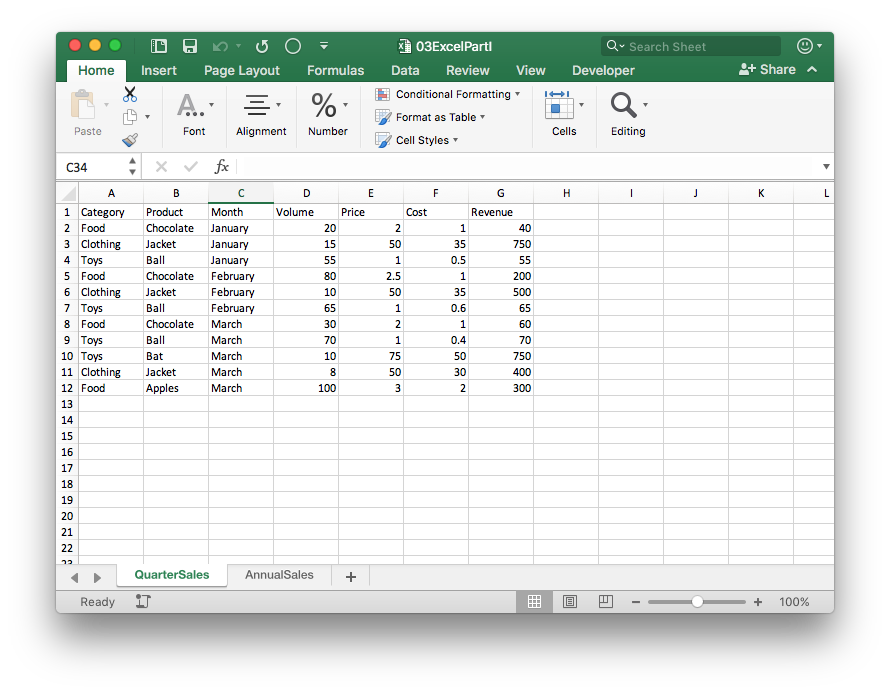
\includegraphics[width=0.9\textwidth]{img/QrSales.png}
%% A complete collection of examples from this lecture can be found in the {\sf 03Excel.xlsx} file on CANVAS.  Demos are saved to {\st DemoPartI.xlsx}
%\end{frame}


\begin{frame}{Excel Ribon}
\begin{description}
\item[ribbon] The Excel ribbon is the strip of icons above the worksheet area. It replaces the menus and toolbars found in Excel 2003 and earlier.
\item[ribbon tab] contains multiple commands logically sub-divided into groups\\
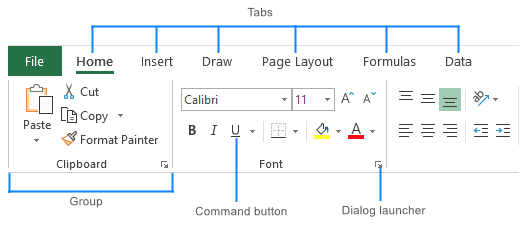
\includegraphics[width=0.6\textwidth]{ribbon} \href{https://www.ablebits.com/office-addins-blog/2019/07/02/excel-ribbon-guide/}{\scriptsize img source}.
\end{description}
\end{frame}





\begin{frame}{Workbook vs. worksheets}
\begin{description}
\item[workbook] A workbook is the name given to an Excel file and contains one or more worksheets.
\medskip
\item[worksheet] A worksheet (or sheet/spreadsheet) is a single page in a file created with an electronic spreadsheet program.
\medskip
\end{description}
For example {\sf 03ExcelPartI.xlsx}  is a \emph{workbook} that contains two \emph{worksheets}.  The name of these worksheets are {\tt QuarterSales} and {\tt AnnualSales}.
\end{frame}



\begin{frame}{Adding and renaming worksheets}
\vfill
To add a new worksheet we simply the plus sign located to the right of the worksheets.
\vspace{-0.5cm}
\begin{center}
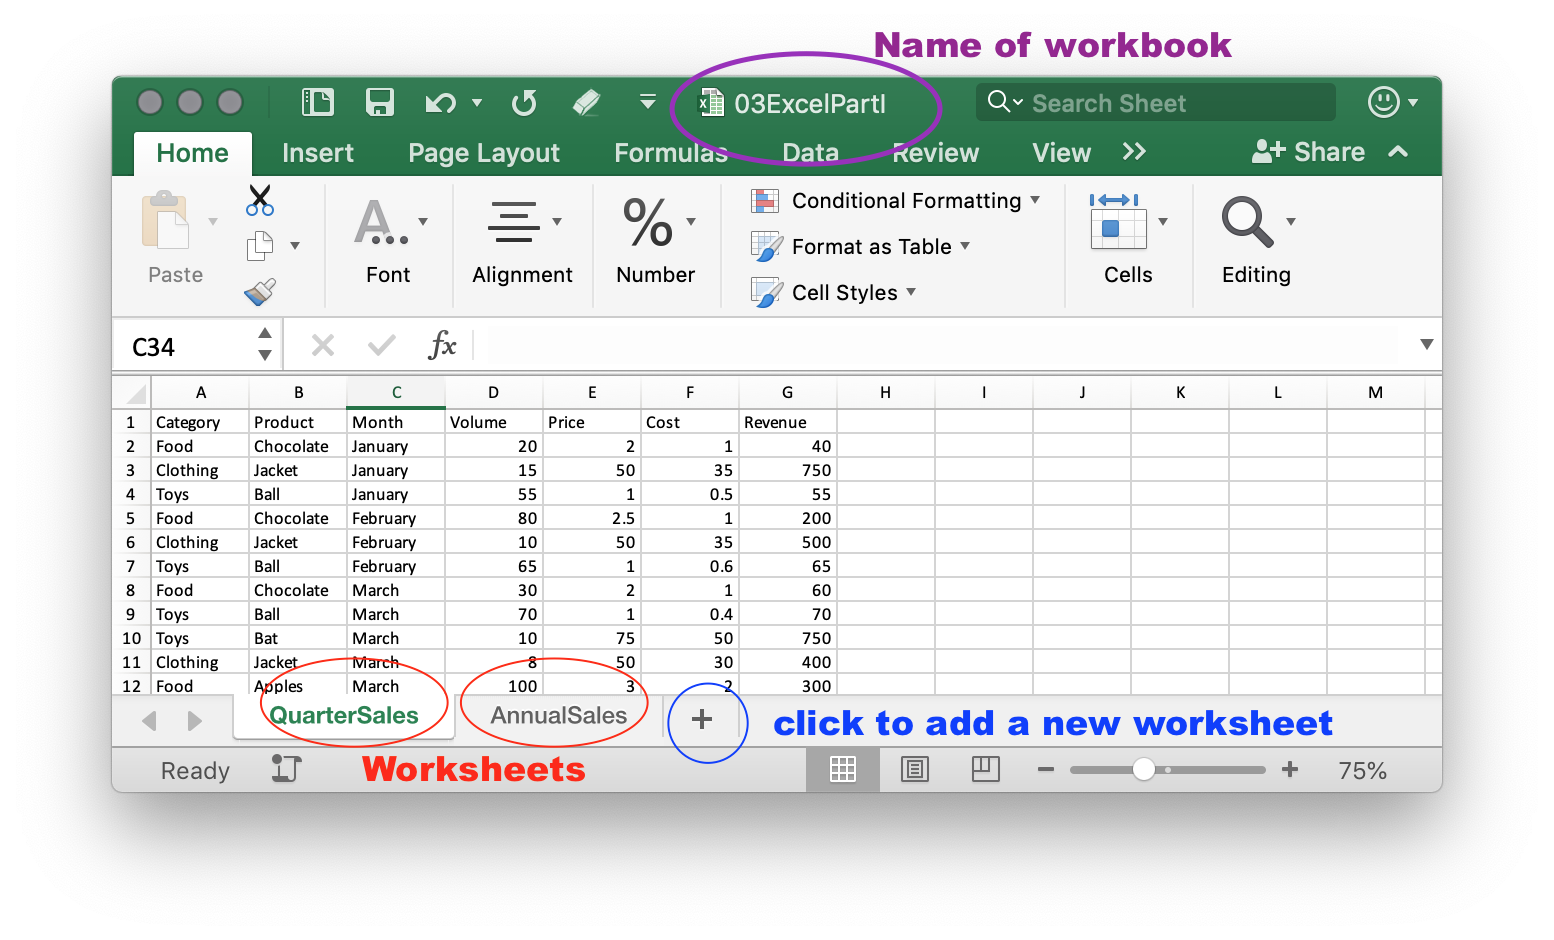
\includegraphics[width=0.86\textwidth]{rename}
\end{center}
\vspace{-0.5cm}
By default, the worksheets are named Sheet1, Sheet2, Sheet3, and so on, but you can change these names by double clicking on the tab and typing an alternate name.
\end{frame}

\begin{frame}
\begin{itemize}
\item To {\bf Move a sheet}, drag the sheet tab to the location that you want along the row of sheet tabs.
\item To {\bf Copy a sheet}
\begin{enumerate}
\item Hold down \keystroke{Ctrl}/\keystroke{Option} (Windows/Mac).
\item Drag the sheet tab to the location that you want the copied sheet to appear along the row of sheet tabs.
\item[\red{Important}] Release the mouse button before you release  \keystroke{Option}/\keystroke{Ctrl}.
\end{enumerate}
\item To move/copy your worksheet to another workbook, you can right click the corresponding worksheet tab and select {\bf Move or Copy}.  Select the desired workbook from the dropdown menu.  Alternatively, you could follow the options outlined \href{https://support.office.com/en-us/article/move-or-copy-worksheets-or-worksheet-data-47207967-bbb2-4e95-9b5c-3c174aa69328}{here}

\end{itemize}

\end{frame}


\begin{frame}{Spreadsheet Addressing}
A \emph{cell} is identified by a column letter and row number.\vspace{2mm}
\hspace*{-6mm}                                                           
 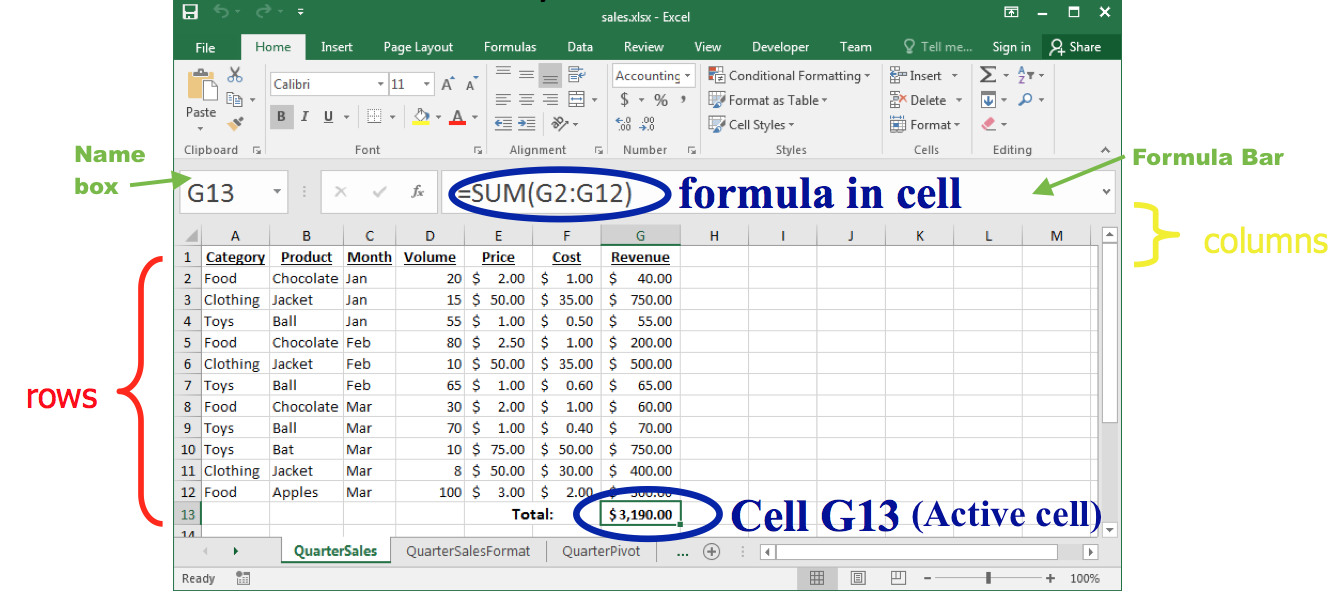
\includegraphics[width=1.1\textwidth]{ExcelSheet.png}
 
 Notice how the  \emph{active cell} (the cell  highlighted by the green rectangle in the spreadsheet) also displays its cell identifier in name box located to the left of the formula bar.
\end{frame}


\begin{frame}{Spreadsheet Addressing}
\begin{itemize}
\item The \emph{rows} in a spreadsheet are \emph{numbered} starting from 1.
\item The \emph{columns} are represented by \emph{letters}.  
\begin{itemize}
\item \textbf A is column 1, \textbf B is column 2, \dots, \textbf Z is column 26, {\bf AA} is column 27, \dots
\end{itemize}
\item  A cell is identified by putting the column letter first then the row number.  
\begin{itemize}
\item e.g. \cell{B3} is the 2nd column and the 3rd row.
\end{itemize}
\end{itemize}
Question: What column number is \textbf{AD}?  How about \textbf{BAD}?
\begin{center}
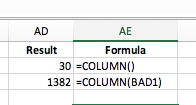
\includegraphics[width=0.4\textwidth]{ColumnRef}
\end{center}
% Answer 30. %https://blog.vishalon.net/excel-column-letter-to-number-quick-reference
\end{frame}


\begin{frame}{Spreadsheet Data Entry}
An entry is added to a cell by clicking on it and typing in the data.  
\begin{itemize}
%\item The data may be a number, text, date, etc. Type and \emph{format} are auto-detected.
\item The spreadsheet attempts to detect the data type and format it
accordingly. It is also possible to manually \emph{format} the data
\begin{center}
 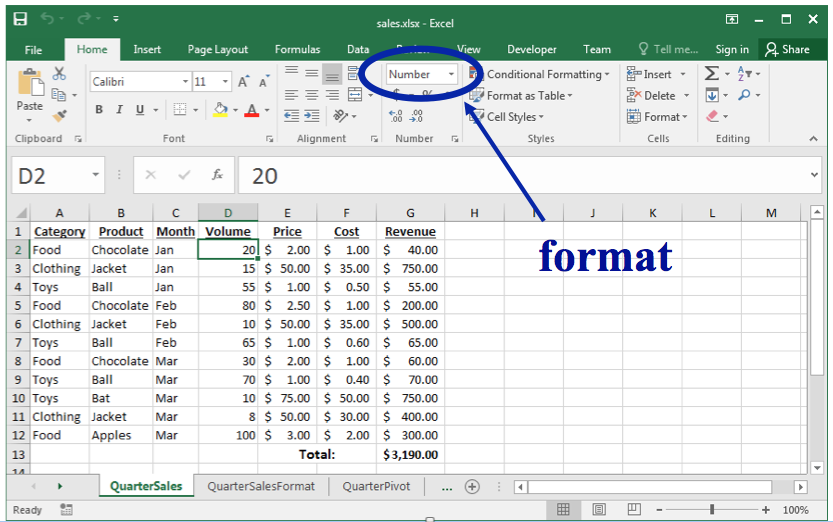
\includegraphics[width=0.8\textwidth]{CellFormat.png}
\end{center}                                         
\end{itemize}
\end{frame}



\begin{frame}{Date and Type Formats}
\begin{itemize}
\item Excel stores dates and time as a date serial number.\medskip
\item The earliest date permitted by Excel is  January 1, 1900 (which has a date serial number equal to 1).
\medskip
\item \href{https://support.office.com/en-us/article/datevalue-function-df8b07d4-7761-4a93-bc33-b7471bbff252}{DATEVALUE()} function converts text to a date serial number which we can then format to display the day however we want
\medskip
\item Alternatively we could use the \href{https://exceljet.net/excel-functions/excel-date-function}{DATE(year, month, day)} function which takes the arguments:
\begin{description}
\item[year] - Number for year.
\item[month] - \textit{Number} for month.
\item[day] - Number for day.
\end{description}
\end{itemize}
% https://www.myonlinetraininghub.com/excel-date-and-time
\end{frame}


%\begin{frame}
%As mentioned before, Excel will try to get the appropriate format of cells.  The various forms below are a few examples of configurations that Excel will automatically  recognize as dates:
%\begin{center}
%\begin{tabular}{|c|c|c|}
%{\bf Entered text} & Excel returns & DATEVALUE \\
%3-1-15 & 
%1-1-09
%1/1/2009
%1/1/09
%1-Jan-09
%1-Jan 09
%1-Jan-2009
%1 Jan 09
%1/1
%\end{tabular}
%\end{center}
%\end{frame}


\begin{frame}{Date and Type Formats}
\begin{itemize}
\item It is important to note that Excel dates require a year, month, \textit{and} day.
\medskip
\item That is, if you are missing a year, for example, Excel won't be able to format that cell as a date unless we provide a year.
\medskip
\item One trick is to give your data an arbitrary year that you hide when you format your cells.
\medskip
\item For example, we could replace {\tt January} with {\tt January 1, 2019} and format the cell to only display the month. 

\begin{center}
\begin{tabular}{|c|c|c|}
\hline
{\bf Cell Format} & {\bf Cell display}& \\
\hline
General &  {\tt January} & (treated as text) \\
Date & {\tt 2019-01-01} & (treated as  serial number 43466)\\
Custom & {\tt January} & (treated as serial number 43466)\\
\hline\end{tabular}
\end{center}
\end{itemize}
\end{frame}
%are recorded with a There's no way to have a date without a year, it's simply a required part of a date. Just like the second is a required part of the time of day - if you enter, say, "1:15", the actual value will be "01:15:00" (or something like that, depending on your regional settings). The only thing you can do is format the column as text, use a date format that hides the year, or tricks like using formulae to extract the day and month into another column and hiding the column with the actual date.
% https://superuser.com/questions/465469/excels-date-format-without-a-year


\begin{frame}{Date and Type Formats}
\begin{itemize}
\item Formatting data helps users read and understand data and is especially important for numbers and dates. 
\item To change the format of a serial date, click the down arrow in the format drop down menu and select {\bf More Number Formats}; this will open up the \textit{Format Cells} pop-up box
\end{itemize}
\begin{center}
 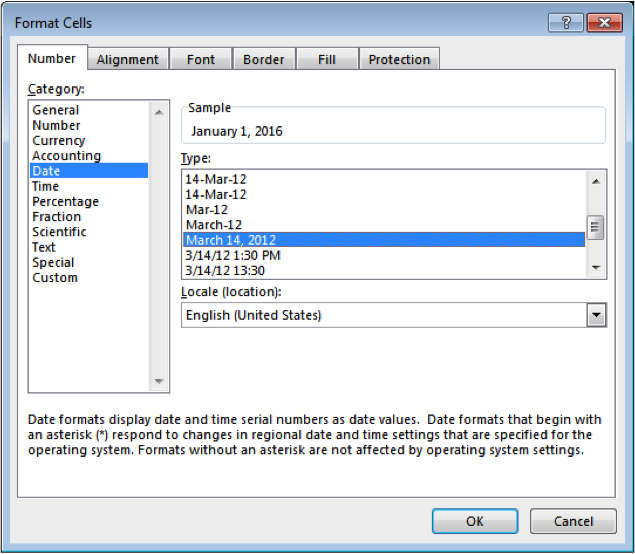
\includegraphics[height=.6\textheight]{DateType}
\end{center}
\end{frame}




\begin{frame}{Date and Type Formats}
\begin{itemize}
\item You can use either built-in or custom formats or  \href{https://www.ablebits.com/office-addins-blog/2015/03/11/change-date-format-excel/\#custom-date-format}{custom formatting} (see a summary of these on the next slide)
\medskip
\item For example, applying the custom format of {\sf dd/mmm-yy} on the 
date \textit{January 1, 2005} would display {\tt 01/Jan-05}.
\medskip
\item You can also accomplish this type of formatting using the \href{https://www.ablebits.com/office-addins-blog/2015/04/08/convert-date-text-excel/}{TEXT()} function.  These cells, however, will be treated as text, not dates. 
\end{itemize}
\end{frame}



\begin{frame}{Custom Date Options}
Here are some examples of custom formatting options. Source: \href{https://www.ablebits.com/office-addins-blog/2015/03/11/change-date-format-excel/\#custom-date-format}{ablebits.com}
\begin{center}
{\bf Example (January 1, 2005)} 
\begin{tabular}{|c|l|l|}
\hline
{\bf Code} & {\bf	Description} & 	{\bf Result}\\
\hline
m	& Month number without a leading zero&	1\\
mm	& Month number with a leading zero	& 01\\
mmm	& Month name, short form	 & Jan\\
mmmm	& Month name, full form& 	January\\
mmmmm &	Month as the first letter	& J \footnote{(stands for January, June and July)}\\
d &	Day number without a leading zero&	1\\
dd&	Day number with a leading zero&	01\\
ddd	&Day of the week, short form&	Mon\\
dddd&	Day of the week, full form	& Monday\\
yy&	Year (last 2 digits)&	05\\
yyyy&	Year (4 digits)	&2005\\
\hline\end{tabular}
\end{center}
\end{frame}





\begin{frame}{Currency vs Accounting}
It is worth mentioning the difference between \textit{Currency} and \textit{Accounting} as they are very similar.
\begin{itemize} 
\item Currency places the dollar sign to the immediate left of the number while Accounting places the dollar sign on the left edge of the cell.
\item Currency displaces zeros as \$0.00 while Accounting denotes zeros with dashes
\item The Accounting format displays negative numbers in parentheses.
\begin{center}
 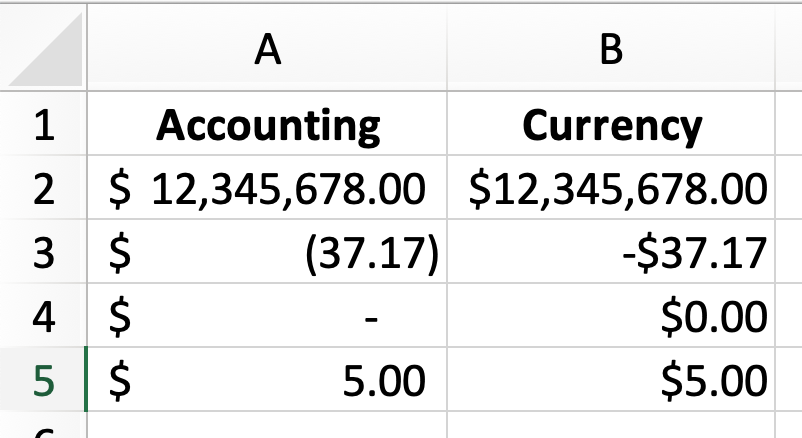
\includegraphics[width=0.4\textwidth]{currencyVsAccounting}
\end{center}                                         
\end{itemize}
\end{frame}



\begin{frame}{Spreadsheet Formatting (Windows)}
A text editor shortcut will allow you to format cells in bold, italics, underline, fonts, colours, justify, etc.
\begin{center}
 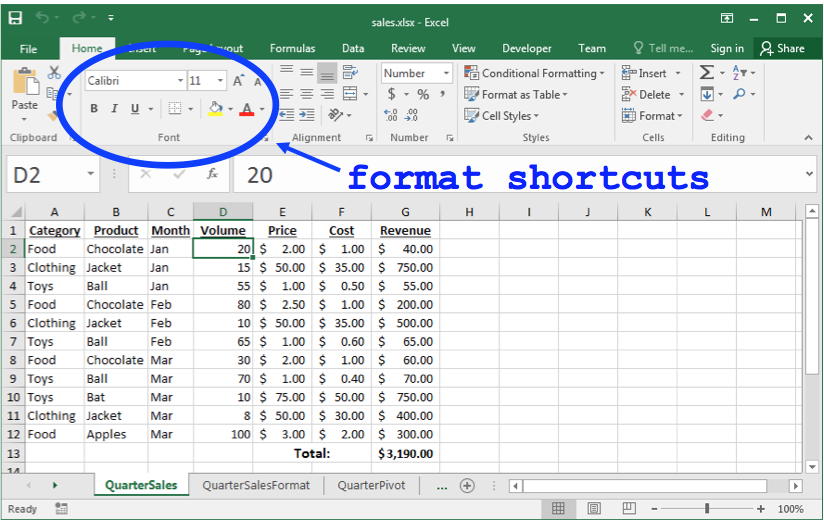
\includegraphics[width=0.8\textwidth]{FormatShortcut.png}
\end{center}                                         
\end{frame}


\begin{frame}{Try It!}
\begin{exampleblock}{Exercise}
Make a copy of the {\tt QuarterSales} worksheet and call it {\tt QuarterSalesFormat}.  Format the headers of the QuarterSales worksheet to be {\bf bold}, \underline{underlined} and centered.
\end{exampleblock}

\begin{exampleblock}{Exercise}
Format all monetary cells to the format \textit{Currency}
\end{exampleblock}


\end{frame}



\begin{frame}{Spreadsheet Selecting Multiple Cells}\label{selectingcells}
There are a number of ways of selecting multiple cells at a time:
\begin{enumerate}
\item With the mouse, (left) click and drag mouse to select a rectangle region of cells.
\item With keyboard, hold \keystroke{SHIFT} key and use arrow keys to select a rectangle region of cells.
\item With mouse and keyboard, while holding \keystroke{CTRL}(windows)/\keystroke{Cmnd}(mac) key, (left) click on individual cells to select non-contiguous cells. 
\item Click on a row number to select a whole row\footnote{or until the first empty cell}  or select the first column in that row and press \keystroke{SHIFT} + \keystroke{Cmnd}/\keystroke{Cntrl} + \keystroke{$\rightarrow$}
\item Click on a column header to select a whole column$^2$ or select the first row in that column and  \keystroke{SHIFT} + \keystroke{Cmnd}/\keystroke{Ctrl} + \keystroke{$\downarrow$}
\end{enumerate}
See more keyboard shortcuts  \href{https://exceljet.net/keyboard-shortcuts}{\textcolor{blue}{here.}} (eg. \ukey + \keystroke{A} 
select entire worksheet) \href{https://youtu.be/L9n3tbufCyk}{See demo}

\end{frame}



\begin{frame}{Range Selecting Cells Example}
\begin{center}
 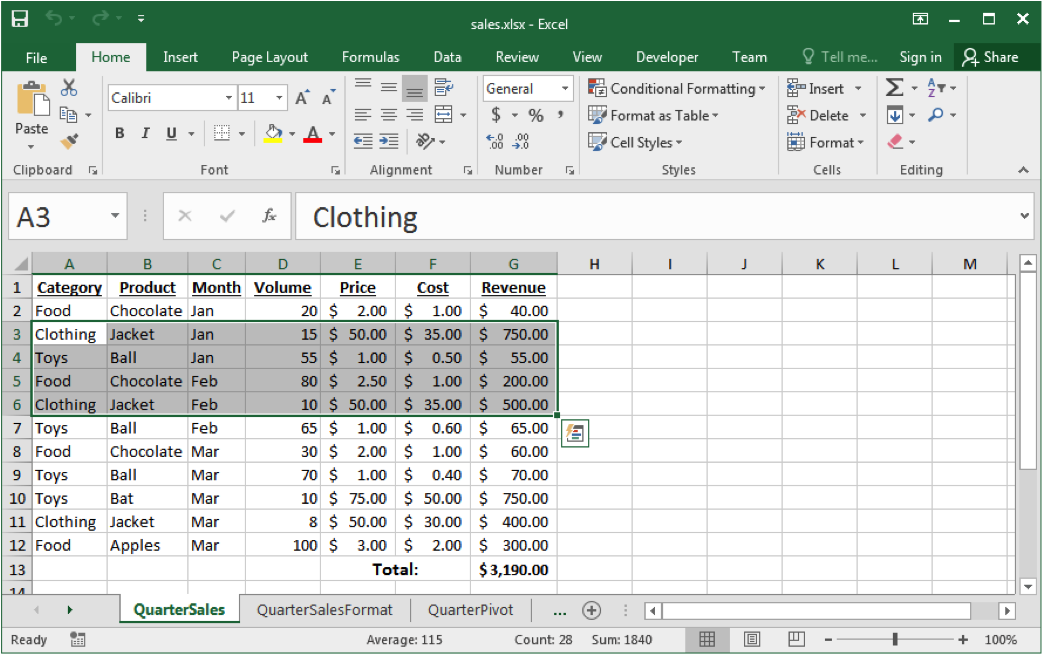
\includegraphics[width=0.8\textwidth]{SelectingCells}
\end{center}                                         
\end{frame}


\begin{frame}{Selecting non-contiguous}
\begin{center}
 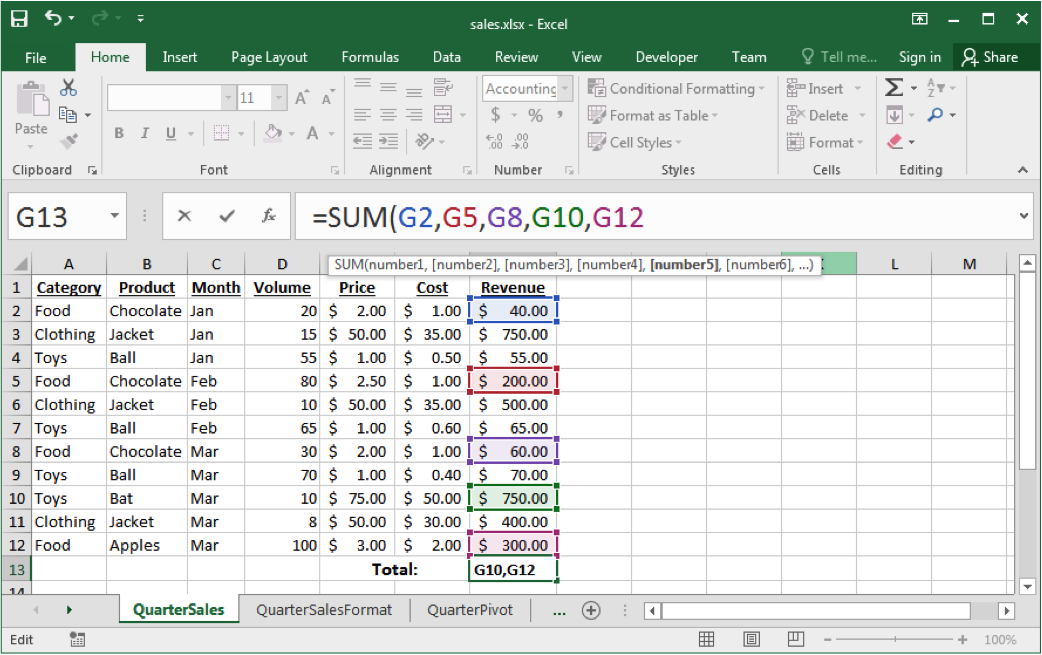
\includegraphics[width=0.8\textwidth]{SelectingIndCells}
\end{center}                                         
\end{frame}

\begin{frame}{Manipulating Cells}
Once you have selected one or more cells, there are several common actions you can perform:
\begin{enumerate}
\item DELETE
\begin{itemize}
\item delete the contents of all cells by pressing \keystroke{delete} key
\item delete the contents and the cell locations (then shift remaining) by selecting Edit menu, Delete\dots or Delete\dots pop-up menu (brought up by right click).
\end{itemize}
\item Cut, Copy, Paste
\begin{itemize}
\item cut - copies selected cells to clipboard and removes from document (\ukey + \keystroke{X})
\item copy - copies selected cells to clipboard (\ukey + \keystroke{C})
\item paste - copies cells in clipboard to sheet starting at currently selected cell  (\ukey + \keystroke{V})
\end{itemize}
\item Add selected cells to a formula (requires that you were previously constructing a formula before selecting the cells).
\end{enumerate}
\end{frame}


\begin{frame}{Cut, Copy, Paste}
Alternatively you could use the command button shortcuts located in the {\bf Home} tab on the ribbon.
\begin{center}
 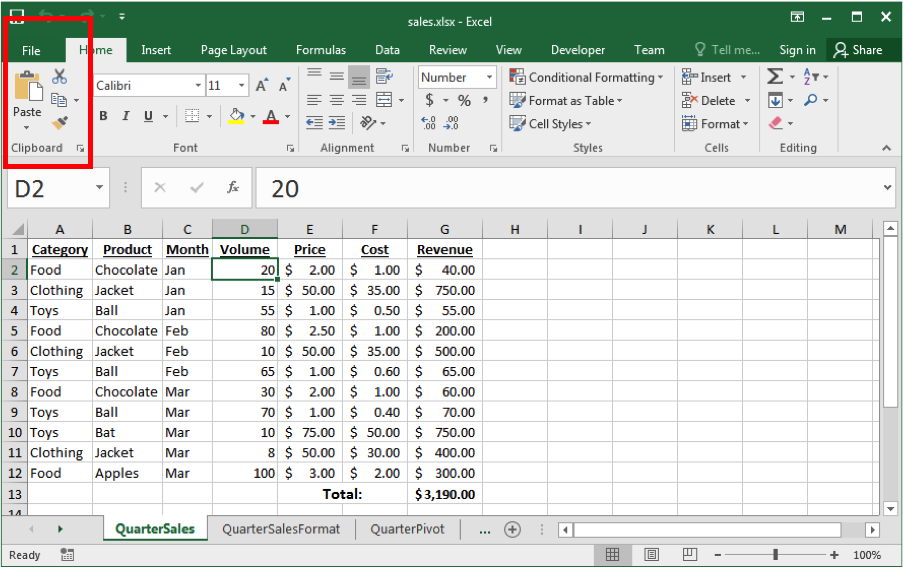
\includegraphics[width=0.9\textwidth]{CutCopyPaste.png}
\end{center}                                         
\end{frame}

\begin{frame}{Paste Button Ribbon}
\begin{itemize}
\item Some buttons in the ribbon open a menu with additional options. 
\item For example, the Paste button  opens a menu with additional pasting options such as {\bf Paste Values}, {\bf Formulas},\dots  which will be useful to us later.
\end{itemize}
\begin{center}
 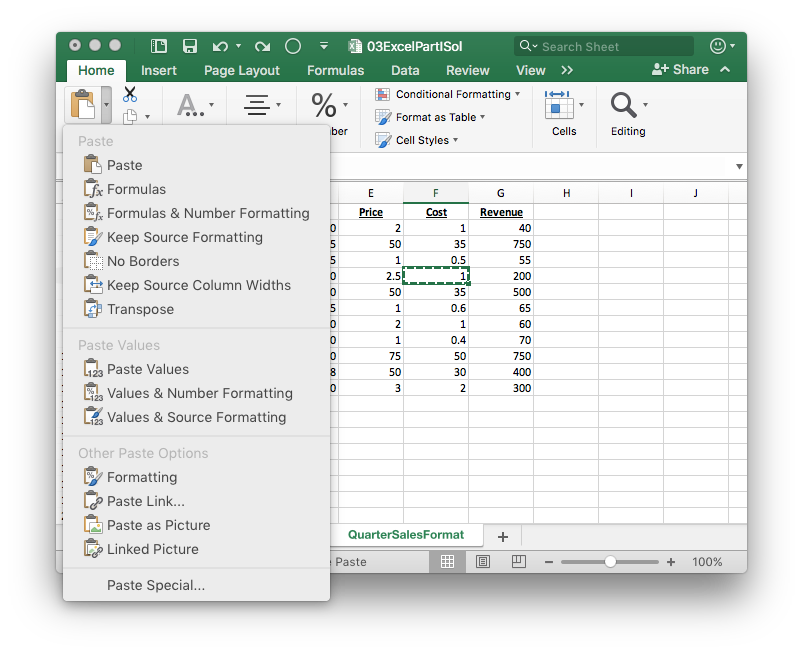
\includegraphics[width=0.8\textwidth]{pasteOpt}
\end{center}                                         

\end{frame}




\begin{frame}{Manipulating Cells - Filling}
\emph{Filling} combines copy and paste.  There is a small box or tab beyond the cell's lower right corner (fill handle).  Grab it with the cursor and pull to other cells. \\
\begin{center}
 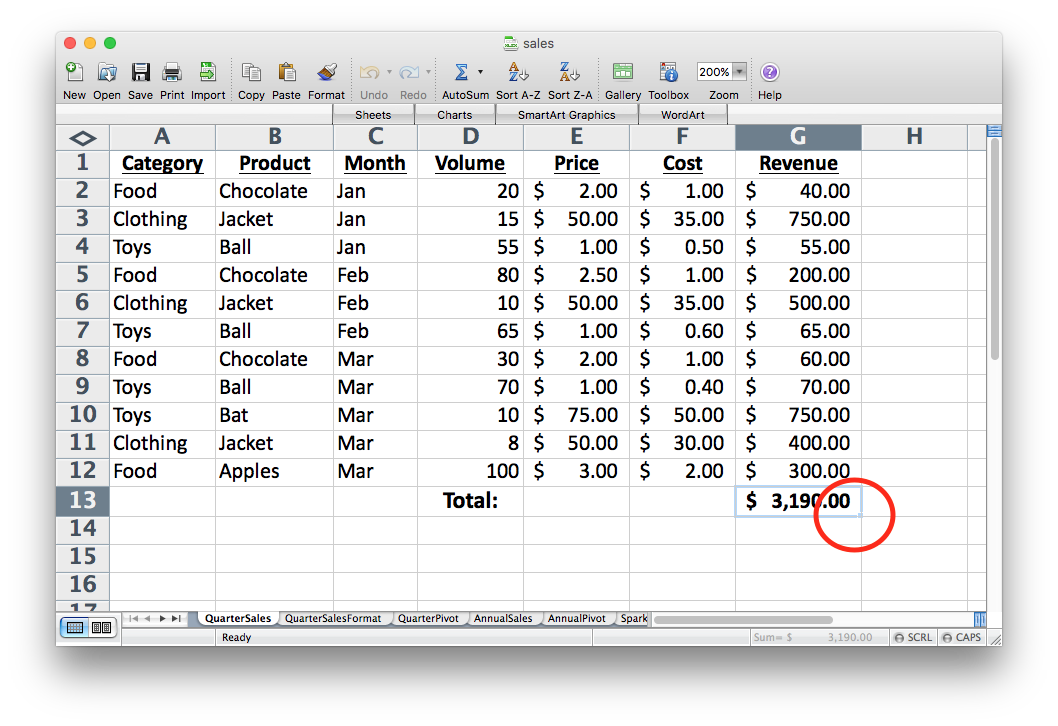
\includegraphics[width=0.8\textwidth]{Filling}
\end{center}
\end{frame}


\begin{frame}{Manipulating Cells - Filling}
 Double clicking that lower corner will quickly copy and paste that formula to the end of the data (or until the first blank row).
\begin{center}
 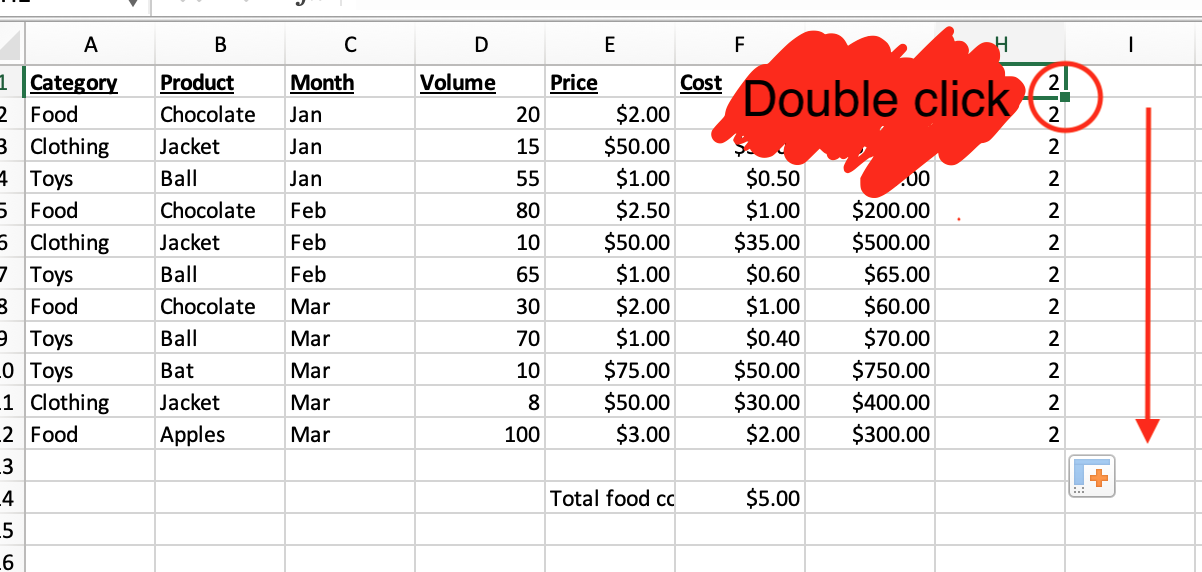
\includegraphics[width=0.9\textwidth]{doubleClick}
\end{center}                                         
%{\bf Warning}: If there are blank cells in your right-mose column it will only extend/fill  until a blank cell appears on its left.                                        
\href{https://youtu.be/O8c9N6CIqWM}{See demo on YouTube}
\end{frame}






\begin{frame}{Hiding Columns and Rows}
You can hide a column or row by  right-clicking on the column or row header and selecting \emph{Hide}.  
\begin{itemize}
\item The column/row still exists but will not be displayed or printed until we select \emph{Unhide}. \href{https://youtu.be/2Z0kPQfhDbE}{Link to my demo on YouTube}
\end{itemize}
\begin{center}
 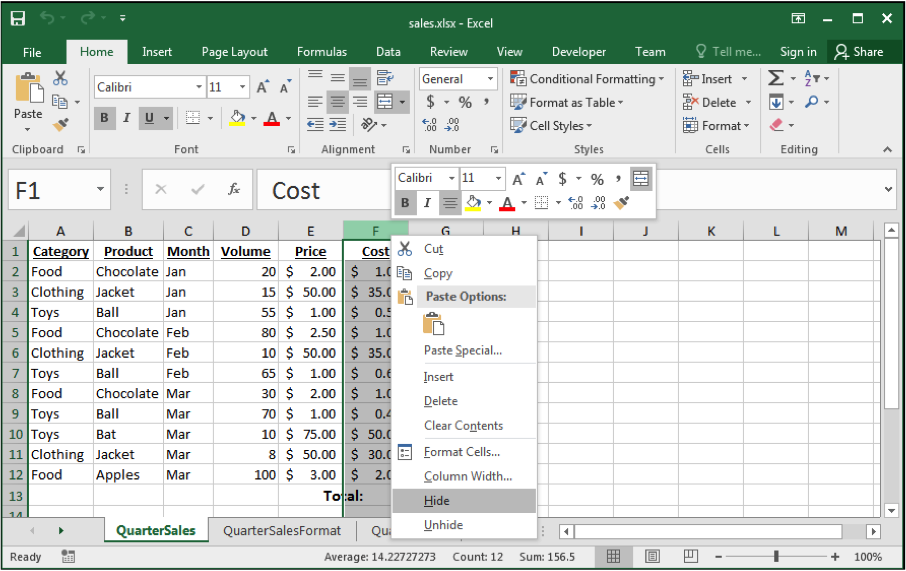
\includegraphics[width=0.8\textwidth]{Hide}
\end{center}                                         
\end{frame}

\begin{frame}{Selecting Cells Question}
\begin{example}
 Which method allows you to select non-contiguous cells in a spreadsheet?
\begin{enumerate}[A)]
\item hold \keystroke{SHIFT} key and use arrow keys 
\item With the mouse left click on a cell and drag mouse 
\item hold \keystroke{CTRL}(windows)/\keystroke{Cmnd}(mac) key and use arrow keys 
\item hold \keystroke{CTRL}(windows)/\keystroke{Cmnd}(mac) key and left click on cells
\end{enumerate}
\end{example}
\end{frame}



\begin{frame}<handout:0>{Selecting Cells Question}
\begin{block}{Answer}
 Which method allows you to select non-contiguous cells in a spreadsheet?
\begin{enumerate}[A)]
\item hold \keystroke{SHIFT} key and use arrow keys 
\item With the mouse left click on a cell and drag mouse 
\item hold \keystroke{CTRL}(windows)/\keystroke{Cmnd}(mac) key and use arrow keys 
\item \answer{hold \keystroke{CTRL}(windows)/\keystroke{Cmnd}(mac) key and left click on cells}
\end{enumerate}
\end{block}
\end{frame}

\begin{frame}{Entering Formulas}
A \emph{formula} is any expression that begins with an equal sign (=).
\begin{itemize}
\item The equal sign means that a calculation must be done to compute the cell value.
\end{itemize}
\begin{center}
 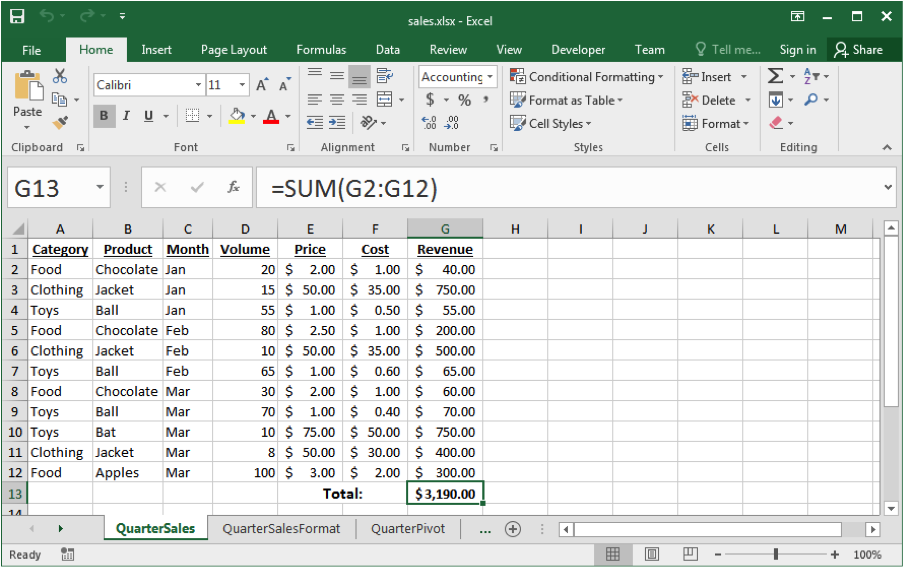
\includegraphics[width=0.8\textwidth]{formula}
\end{center}                                         
\end{frame}

\begin{frame}[fragile]{Formula Expressions}
A formula expression can consist of literals (numbers, text strings), operators, functions (eg. MAX(), AVERAGE()), and cell references.\par \vspace{3mm}  
Simple mathematical expressions:
\begin{itemize}
\item {\tt = 1 + 5}
\item {\tt = 1.5 * 3.14 + 42}
\end{itemize}
Common functions: 
\begin{itemize}
\item  \verb|= ROUND(PI(),2)			// Result is 3.14|
\item = \verb|CONCATENATE("Hello", " World")	// Hello World|
\end{itemize}
Other common functions for trigonometry, dates, and finance are available. See a full list of functions \href{https://support.office.com/en-us/article/excel-functions-alphabetical-b3944572-255d-4efb-bb96-c6d90033e188}{here}
\end{frame}


\begin{frame}{Using Formulas}
\begin{itemize}
\item In order to use functions correctly, you need to follow a certain structure, or \emph{syntax}.
\medskip
\item The basic syntax for a function is the equals sign (=), the function name (eg, SUM), and one or more \emph{arguments}/\emph{inputs} within parenthesis. For example:
\begin{center}
{\tt =SUM(1,2,3)}
\end{center}
Once we press \keystroke{ENTER} (or leave the cell), it will display the 
result, i.e. \emph{output},  of the formula (in this case is {\tt 6}).  Returning to that cell will display the formula in the formula bar.
\medskip
\item N.B. if you function has no arguments, you will still need to type the parenthesis.  For example 
{\tt =NOW()}
returns the current date and time as output.  
\end{itemize}
\end{frame}

\begin{frame}[fragile]{Using Excel Functions}
\begin{itemize}
\item You can get help on any function by searching its name in Excel's drop down Help menu
\end{itemize}
\begin{center}
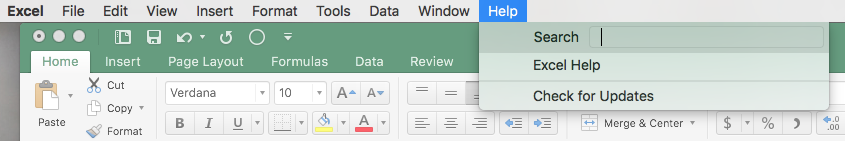
\includegraphics[width=0.8\textwidth]{img/Help.png}
\end{center}
\begin{itemize}
\item Alternatively, you can navigate to the {\bf Formulas} tab in the ribbon and select the 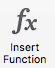
\includegraphics[height=2em]{insertfunction} button (there is also a shortcut to this button directly beside the formula bar 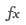
\includegraphics[height=1.em]{ficon}).  This will bring up a {\bf Formula Builder} window which contains the name of all the functions in Excel, with a search and description on how to use each function. 
\end{itemize}
\end{frame}



\begin{frame}[fragile]{Arrays}
Alternatively we could have created an array using \{\} to compute our sum:
\begin{verbatim}
=SUM({1,2,3})
\end{verbatim}
This is equivalent to the following calculation:
\begin{center}
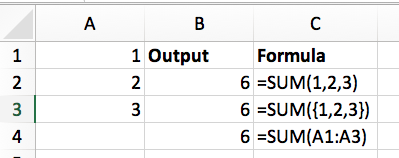
\includegraphics[width=0.4\textwidth]{img/sumarray.png}
\end{center}
These examples and others can be found in {\bf DemoPartI.xlsx} on Canvas
\end{frame}


% Excel functions:
% https://edu.gcfglobal.org/en/excel2016/functions/1/

\begin{frame}{Cell Referencing}
The power of formulas comes from using cell references (similar to variable names in programming). \par \vspace{3mm}  

Cell reference examples: 
\begin{itemize}
\item {\tt = \cell{A1} + \cell{A2}}
\item {\tt = \cell{B1} + \cell{A3} - \cell{A4}}
\end{itemize}
\medskip
Cell address will appear in different coloured font within your formula for ease of viewing.  In addition, the cell itself will be outlined with the same colour when the formula is selected.
\begin{center}
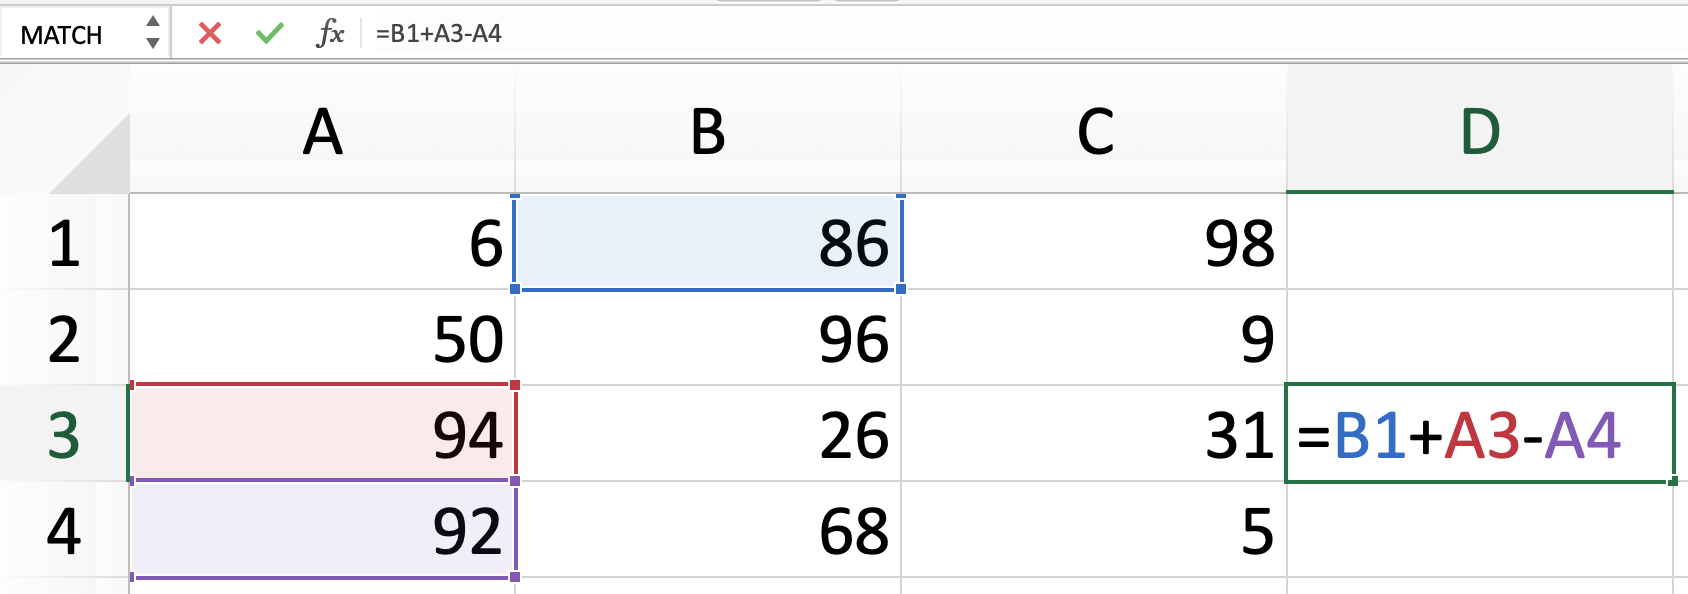
\includegraphics[width=0.7\textwidth]{img/colours}
\end{center}
\end{frame}


\begin{frame}{Cell Referencing}{}
{\bf TIP} Rather than typing out cell names while constructing a formula, you can select them using your mouse or keyboard as done on  \hyperlink{selectingcells}{this} slide.
You can refer to a single cell, a range of cells, a location in another worksheet, or a location in another workbook.
\begin{figure}[htbp]
\begin{center}
\caption{Example of using cell references across worksheets. General syntax: {\tt <SheetName>!<CellAddress>}}
\vspace{-1em}
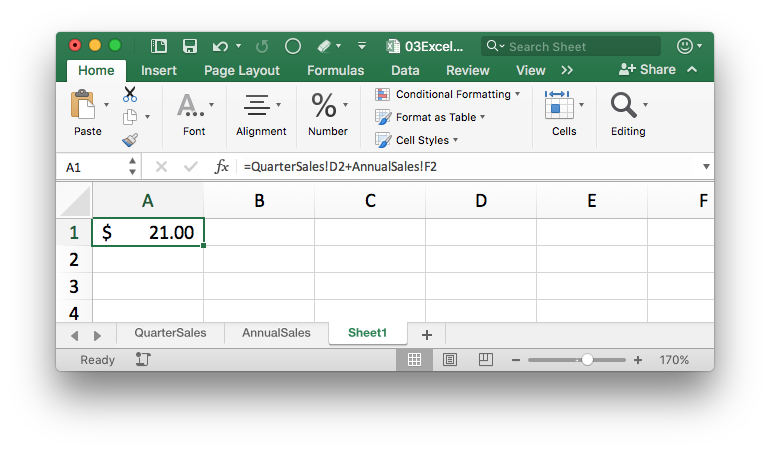
\includegraphics[width=0.9\textwidth]{img/cellref}
\label{default}
\end{center}
\end{figure}
\end{frame}

\begin{frame}{Formula Questions}
Excel follows the BEDMAS order or operations (Brackets, Exponents, Division, Multiplication, Addition, Subtraction). % where does modulo fit?
\begin{example}
{Question:} A cell contains the following: {\tt=2+4*3}  What is the value of the cell?
\begin{enumerate}[A)]
\item 14
\item 18
\item =2+4*3
\item None of the above
\end{enumerate}
\end{example}
\end{frame}

\begin{frame}<handout:0>{Formula Questions}
\begin{block}
{Answer:} A cell contains the following: {\tt=2+4*3}  What is the value of the cell?
\begin{enumerate}[A)]
\item \textbf<1>{\textit<1>{{\color<1>{iyellow}{14}}}}
\item 18
\item =2+4*3
\item None of the above
\end{enumerate}
\end{block}
\end{frame}

\begin{frame}[fragile]{Formula Questions}
Excel follows the BEDMAS order or operations (Brackets, Exponents, Division, Multiplication, Addition, Subtraction). % where does modulo fit?
\begin{example}
{Question:} A cell contains the following: \verb|=(2+4)*3^2|  What is the value of the cell?
\begin{enumerate}[A)]
\item 38
\item 54
\item 324
\item None of the above
\end{enumerate}
\end{example}
\end{frame}

\begin{frame}<handout:0>[fragile]{Formula Questions}
\begin{block}
{Answer:} A cell contains the following: \verb|=(2+4)*3^2|  What is the value of the cell?
\begin{enumerate}[A)]
\item 38
\item \answer{54}
\item 324
\item None of the above
\end{enumerate}
\end{block}
\end{frame}



\begin{frame}[fragile]{Using Excel Functions}
\begin{itemize}
\item Excel will attempt to autocomplete your formulas.
\medskip
\item To accept a suggestion, press \keystroke{TAB}.
\medskip
\item Excel will provide a guideline of how the function is used in the lower right corner of the cell.  Optional arguments appear in square brackets \verb|[]|
\begin{center}
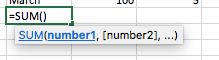
\includegraphics[width=0.4\textwidth]{img/sum.png}
\end{center}
\end{itemize}
\end{frame}




\begin{frame}{Using Excel Functions}
For example, in \cell{H6} we have {\tt =POWER(G2,2)} = $25^2$ = \texttt{625}. {\tt POWER} is the function and {\tt G2} and {\tt 2} are the inputs and 625 is the output.
\begin{center}
 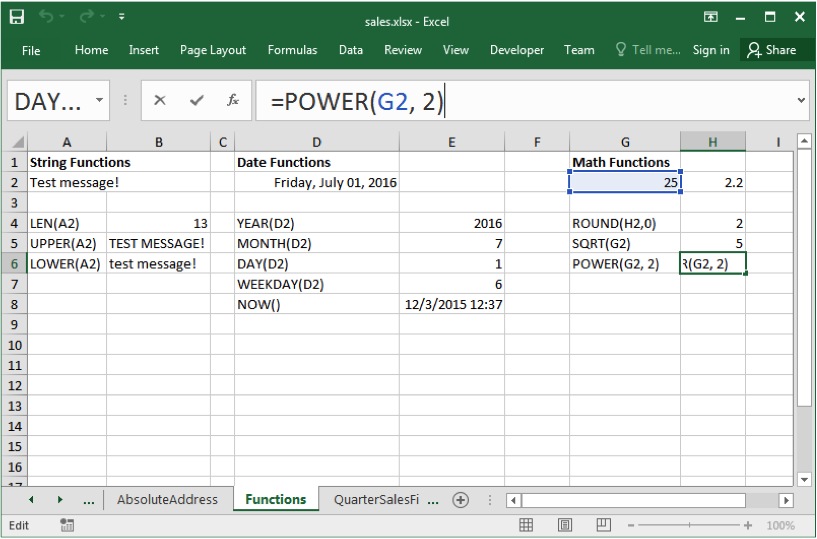
\includegraphics[width=0.8\textwidth]{function}
\end{center}
\end{frame}

\begin{frame}{Try Entering Formulas}
  \begin{exampleblock}{Exercise}
Calculate the total Revenue in cell \cell{G13}.  Add the label of {\bf Total Revenue:} to cell \cell{F13}.
 \end{exampleblock}
 {\bf Tip:} Try using the 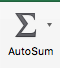
\includegraphics[height=2em]{autosum}  button (located in the {\bf Formula} tab in the ribbon)  to save time! {\bf Directions:}  Select a cell next to the numbers you want to sum (or simply select cell \cell{G13}, click the AutoSum button, then press \keystroke{Enter}.
\end{frame}



\begin{frame}{Try Entering Formulas}
  \begin{exampleblock}{Exercise}
 Add a column for expenses and profit as below. (Expense is volume multiplied by cost and profit is revenue minus expense).
  \end{exampleblock}
\begin{center}
 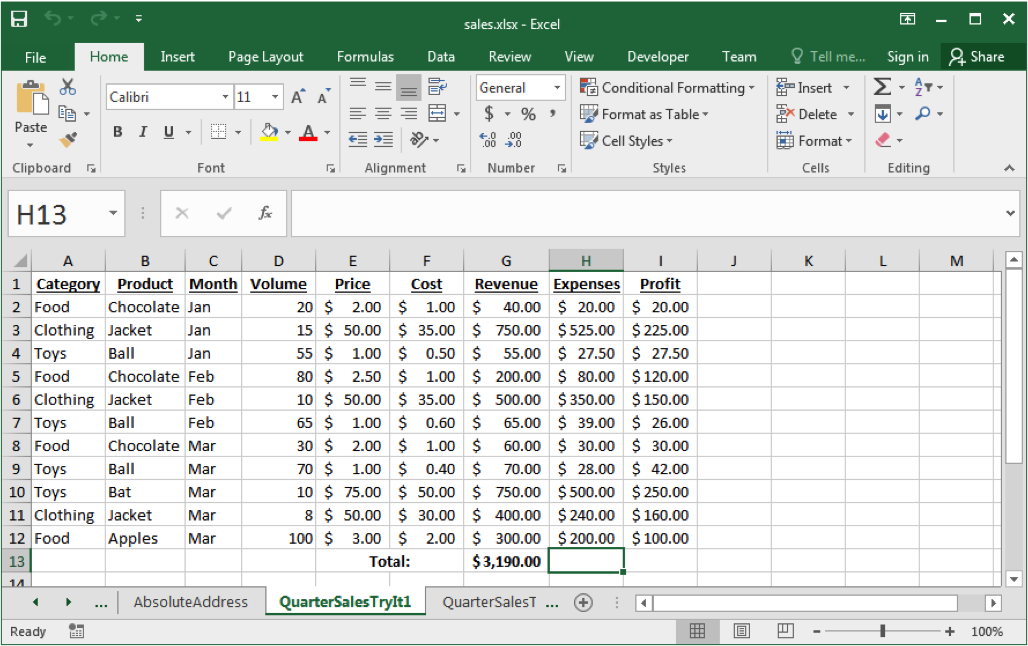
\includegraphics[width=.9\textwidth]{QuarterSalesTryIt.png}
\end{center}
\end{frame}



\begin{frame}[fragile]{Concatenation}
\emph{String concatenation} is when two or more strings are combined by appending them in order.  
The function to do this in Excel is \verb|CONCATENATE()| or \verb|&| operator.
\begin{center}
\hspace*{-9mm}                                                           
 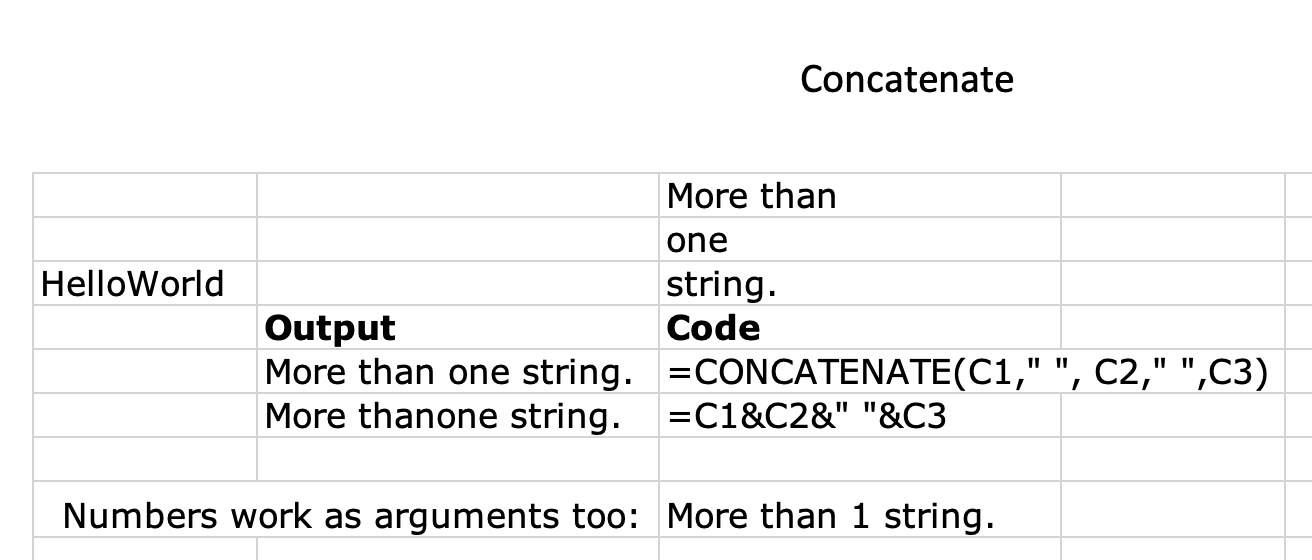
\includegraphics[width=0.8\textwidth]{concatenate}
\end{center}  
Notice that we needed to add spaces \verb|" "| in order for the words to be separated.  In addition, numbers work as arguments too!                                   
\end{frame}

\begin{frame}{Titles and Merged Cells}
\begin{itemize}
\item On the previous slide I added a title to my spreadsheet.  To do this:
\begin{enumerate}
\item Click {\bf View} from the toolbar menu and select {\bf Header and Footer}.
\item Click on the {\bf Add Header} box and insert the desired text.
\item To return to the default view, click {\bf View} from the toolbar menu and select {\bf Normal}. 
\end{enumerate}
\item I also utilize the merge cell option in order to  center text  over a  section of a spreadsheet. To do this:
\begin{enumerate}
\item Highlight or select a range of cells.
\item Right-click on the highlighted cells and select Format Cells....
\item Click the Alignment tab and place a checkmark in the checkbox labeled Merge cells.
\end{enumerate}
Alternatively, you can merge and center a group of cells  using  the Merge and Center button 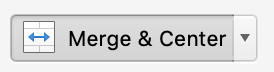
\includegraphics[height=1.5em]{mergeandcenter} located on the Home tab.
\end{itemize}
\end{frame}




\begin{frame}[fragile]{Formulas Question}
\begin{example}
 A cell contains the following: \verb|='ABC'+'DEF'|. What is the value of the cell?
\begin{enumerate}[A)]
\item  error
\item  ABCDEF
\item  'ABC'+'DEF'
\end{enumerate}
\end{example}
\end{frame}



\begin{frame}<handout:0>[fragile]{Formulas Question}
\begin{block}{Answer}
 A cell contains the following: \verb|='ABC'+'DEF'|. What is the value of the cell?
\begin{enumerate}[A)]
\item  \answer{error}
\item  ABCDEF
\item  'ABC'+'DEF'
\end{enumerate}
\end{block}
\end{frame}


\begin{frame}[fragile]{\texttt{LOOKUP} function}
\begin{itemize}
\item  The \verb|LOOKUP| function searches for a value in either a row (or column) and returns a corresponding value from a neighbouring row (or column).
\begin{itemize}
\item This function works like searching for numbers in a phonebook: by searching for their name in the phonebook, you can determine their listed phone number.
\end{itemize}
\medskip
\item \verb|VLOOKUP| %searches a column \underline{in a table} ()
does the same thing, only it is restricted to \blue{V}ertical (column) searches
\medskip
\item \verb|HLOOKUP| on the other hand, is restricted to \blue{H}orizontal (row) searches %searches a row \underline{in a table} 
\medskip
\item Some consider  \href{https://support.office.com/en-us/article/lookup-function-446d94af-663b-451d-8251-369d5e3864cb}{LOOKUP} as better than VLOOKUP \href{https://corporatefinanceinstitute.com/resources/excel/functions/lookup-vs-vlookup/}{[Source]}
while others consider \href{https://support.office.com/en-us/article/video-vlookup-when-and-how-to-use-it-9a86157a-5542-4148-a536-724823014785}{VLOOKUP}  is  an improved version of LOOKUP [\href{https://support.office.com/en-us/article/LOOKUP-function-446D94AF-663B-451D-8251-369D5E3864CB}{Source}].  
\medskip
\item We will go through the advantages and disadvantages of each.
\end{itemize}



\end{frame}


\begin{frame}[fragile]{\texttt{LOOKUP} function}
The {\tt LOOKUP} function has the following form:
\verb|LOOKUP(lookup_value, lookup_vector, [result_vector])|
\begin{itemize}
\item {\tt lookup\_value} is the value we would like to match (eg. the name in our phonebook analogy)
\item {\tt lookup\_vector} the corresponding \underline{column} (or row) containing the values from which we are searching for {\tt lookup\_vector} (eg. the column of names in our phonebook analogy)
\item {\tt result\_vector} the corresponding \underline{column} (or row) containing the information we are trying to obtain (eg. the column of phone numbers in our phonebook analogy); this has to be the same size as the {\tt lookup\_vector}
\end{itemize}
\end{frame}

\begin{frame}[fragile]{\texttt{LOOKUP} function}
It is common that we store the {\tt lookup\_value} in a cell so that we might change it easily for future use of the formula.
\begin{center}
 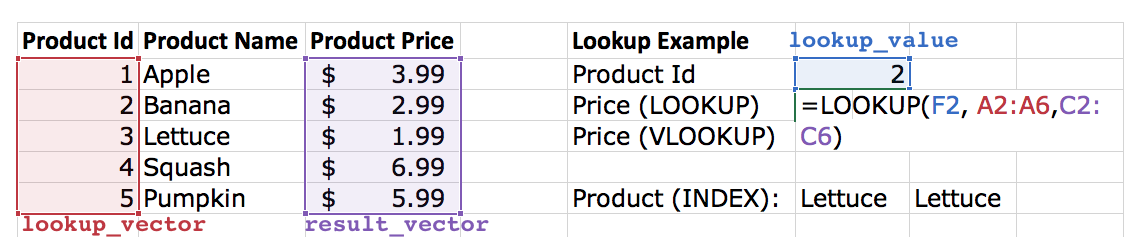
\includegraphics[width=0.96\textwidth]{lookupZoom}
\end{center}
{\bf Formula:} {\tt =LOOKUP(F2, A2:A6,C2:C6)}\\
{\bf Output:} {\tt \$2.99}\\
%Useful \href{https://www.youtube.com/watch?v=E7gQ-PgYkMc}{\blue{YouTube video}}
%\begin{alertblock}
%Important: The values in lookup_vector must be placed in ascending order%: ..., -2, -1, 0, 1, 2, ..., A-Z, FALSE, TRUE; 
%otherwise, LOOKUP might not return the correct value. Uppercase and lowercase text are equivalent. \href{https://support.office.com/en-us/article/LOOKUP-function-446D94AF-663B-451D-8251-369D5E3864CB}{More here}
%\end{alertblock}
\href{https://youtu.be/jvcK_nbxCZM}{YouTube Demo}
\end{frame}


\begin{frame}[fragile]{A comment on \texttt{LOOKUP} function}
\begin{alertblock}{Important}
\begin{itemize}
\item The values in {\tt lookup\_vector} must be placed in {\bf ascending order}: \dots, -2, -1, 0, 1, 2, ..., A-Z, FALSE, TRUE; 
otherwise, LOOKUP might not return the correct value. 
\item Uppercase and lowercase text are treated as equivalent.
\end{itemize}
\end{alertblock}
\begin{example}
Use the lookup function to determine the product ID of a certain product name.
\begin{enumerate}
\item What happens when you try and look up the ID of \textit{Pumpkin}?  
\item How can we fix this problem?
\end{enumerate}
\end{example}

\end{frame}


\begin{frame}[fragile]{\texttt{VLOOKUP} function}
%The {\tt VLOOKUP} function has the following form:
\begin{verbatim}
VLOOKUP(lookup_value, table_array, col_index_num,
 [range_lookup])
\end{verbatim}
\begin{itemize}
\item {\tt lookup\_value} is the value we would like to match (eg. the name in our phonebook analogy)
\item {\tt table\_array} the corresponding \underline{array} (or matrix) containing the values from which we are searching for {\bf and} the information we are trying to obtain. (eg. a matrix contain the columns of names {\bf and} phone numbers in our phonebook analogy)
\item {\tt col\_index\_num} corresponding to the column number containing the information we are trying to obtain (eg. the column of phone numbers in our phonebook analogy)
\item {\tt range\_lookup} An [optional argument] indicating if you want exact (FALSE) or approximate (TRUE (default)) matching.
\end{itemize}
\end{frame}



\begin{frame}[fragile]{\texttt{VLOOKUP} function}
\begin{center}
 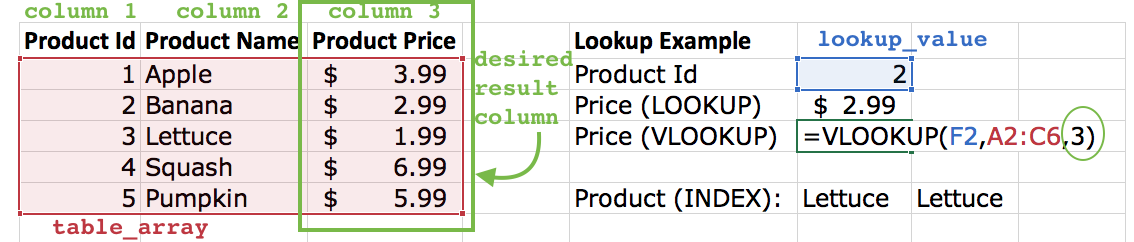
\includegraphics[width=0.96\textwidth]{img/vlookupZoom.png}
\end{center}
{\bf Formula:} {\tt =VLOOKUP(F2,A2:C6,3)}\\
{\bf Output:} {\tt \$2.99}\\
\href{https://youtu.be/q575W8vM7FY}{Youtube Demo}
\end{frame}


\begin{frame}{\texttt{VLOOKUP} function}
  \begin{alertblock}{
  Some warnings about {\tt VLOOKUP}}
    \begin{itemize}
    \item 
    The column of lookup values (the equivalent {\tt lookup\_vector} from the {\tt LOOKUP} example) is expected to be in the left-most column of the {\tt table\_array}.
%    The \texttt{lookup\_value} must appear on the left-most column of the \texttt{table\_array}
    \item If the fourth optional argument \texttt{range\_lookup} is left blank, it defaults to TRUE
    \begin{itemize}
    \item FALSE allows only exact matches while TRUE allows for partial matches
    \end{itemize}
\item If {\tt range\_lookup} is TRUE (the default setting) the first row of the table must be sorted in ascending order. Otherwise, VLOOKUP may return an incorrect or unexpected value.
    \end{itemize}
  \end{alertblock}
N.B. {\tt HLOOKUP} works in the exact same way as {\tt VLOOKUP} only now we look across rows instead of columns.
\end{frame}


\begin{frame}[fragile]{\texttt{VLOOKUP} function}
\begin{center}
 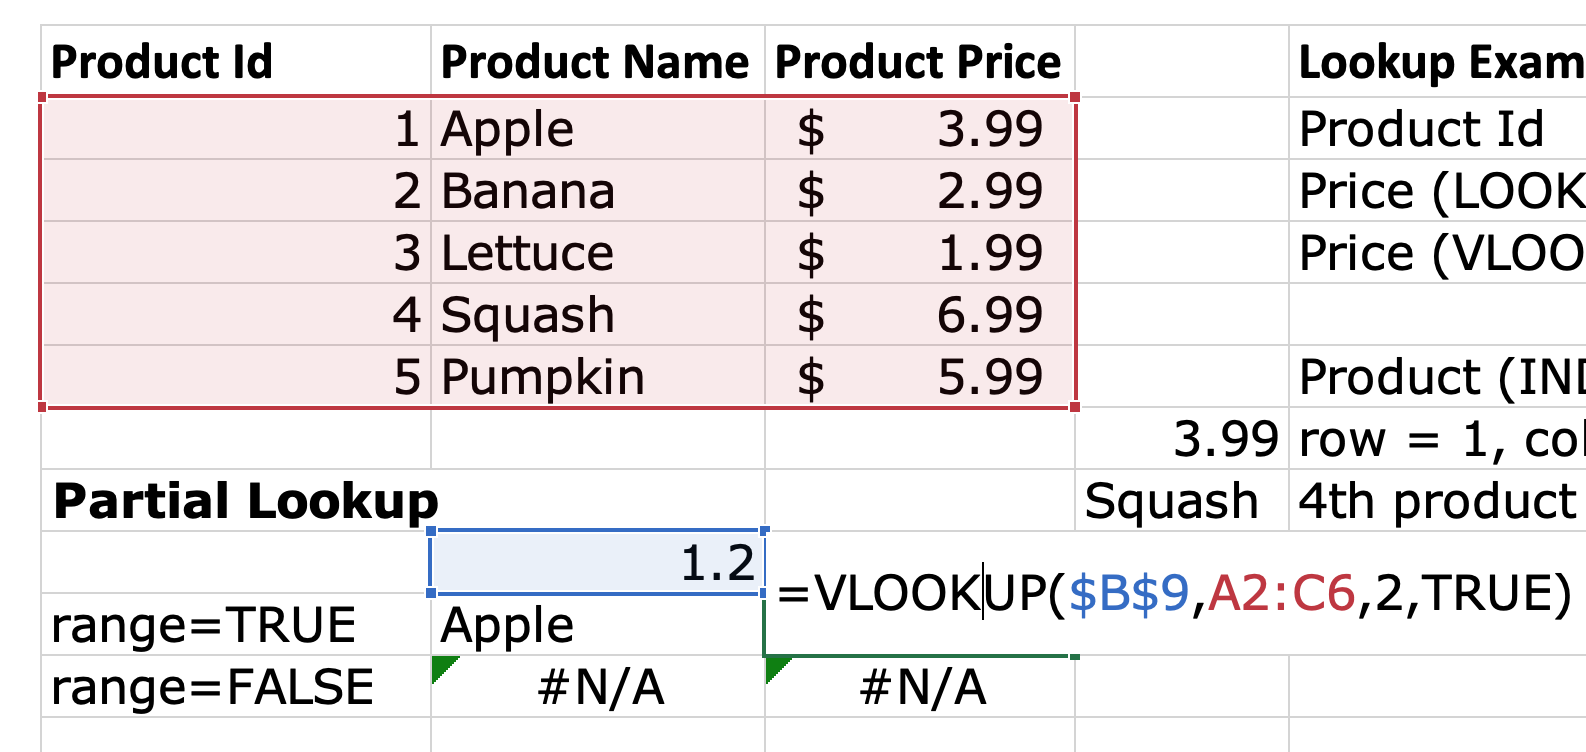
\includegraphics[width=0.96\textwidth]{img/partialLookupZoom}
\end{center}
{\small
{\bf Formula:} {\tt =VLOOKUP(B9,A2:C6,2,TRUE\footnote{\textbf{N.B} doesn't look for the "nearest" value but the greatest value smaller than or equal to the lookup value.})} where \cell{B9} = {\tt 1.2}\\
{\bf Output:} {\tt Apple}\\
{\bf Formula:} {\tt =VLOOKUP(B9,A2:C6,2,FALSE)} where \cell{B9} = {\tt 1.2}\\
{\bf Output:} {\tt \#N/A}}

%, so effectively rounding downs.
\end{frame}

\begin{frame}
\begin{example}
\begin{enumerate}
\item Can you use vlookup function to determine the product ID of a certain product name?
\item Use vlookup function to determine the price a certain product name.  Use the default setting of {\tt range\_lookup = TRUE}? 
\item Test this function with the entry: \textit{Pumpkin}.
\item Test this function with the entry: \textit{Pumpkin}, this time using {\tt range\_lookup = FALSE} 
\end{enumerate}
\end{example}

\end{frame}



\begin{frame}[fragile]{LOOKUP vs. VLOOKUP}

The pros (left) and cons (right) of LOOKUP
%\begin{multicols}{2}
%\begin{description}
%\item[Pros]
%\item[Cons]
%\end{description}
%    \end{multicols}
\begin{multicols}{2}
    \begin{itemize}
        \item  Accommodates left-to-right and right-to-left lookups
        \item  Less restrictive in terms of {\tt lookup/result\_vector}
        \item  Requires ascending ordered {\tt lookup\_vector}
        \item  Partial matching (no option to for exact matches)
    \end{itemize}
    \end{multicols}
    
The pros (left) and cons (right)  of VLOOKUP
\begin{multicols}{2}
    \begin{itemize}
            \item  option to force exact matches
        \item[] 
        \item[] 
        \item[]
                 \item Accommodates only  left-to-right lookups
        \item Requires a table (more restrictive) 
        \item Requires ascending ordered {\tt lookup\_vector}
    \end{itemize}
    \end{multicols}
Both have unexpected behaviour with duplicates 
\end{frame}


\begin{frame}[fragile]{\texttt{INDEX} function}
The syntax for the INDEX function in Microsoft Excel is:
$$\verb|INDEX( table, row_number, column_number )|$$
It returns the value from within a table or range (i.e. an array of cells) at the given index. (Think of indexing a matrix in {\sf R} using {\tt mat[i,j]} with {\tt i} is your {\tt row\_number} and {\tt j} is your {\tt col\_number})
\begin{center}
 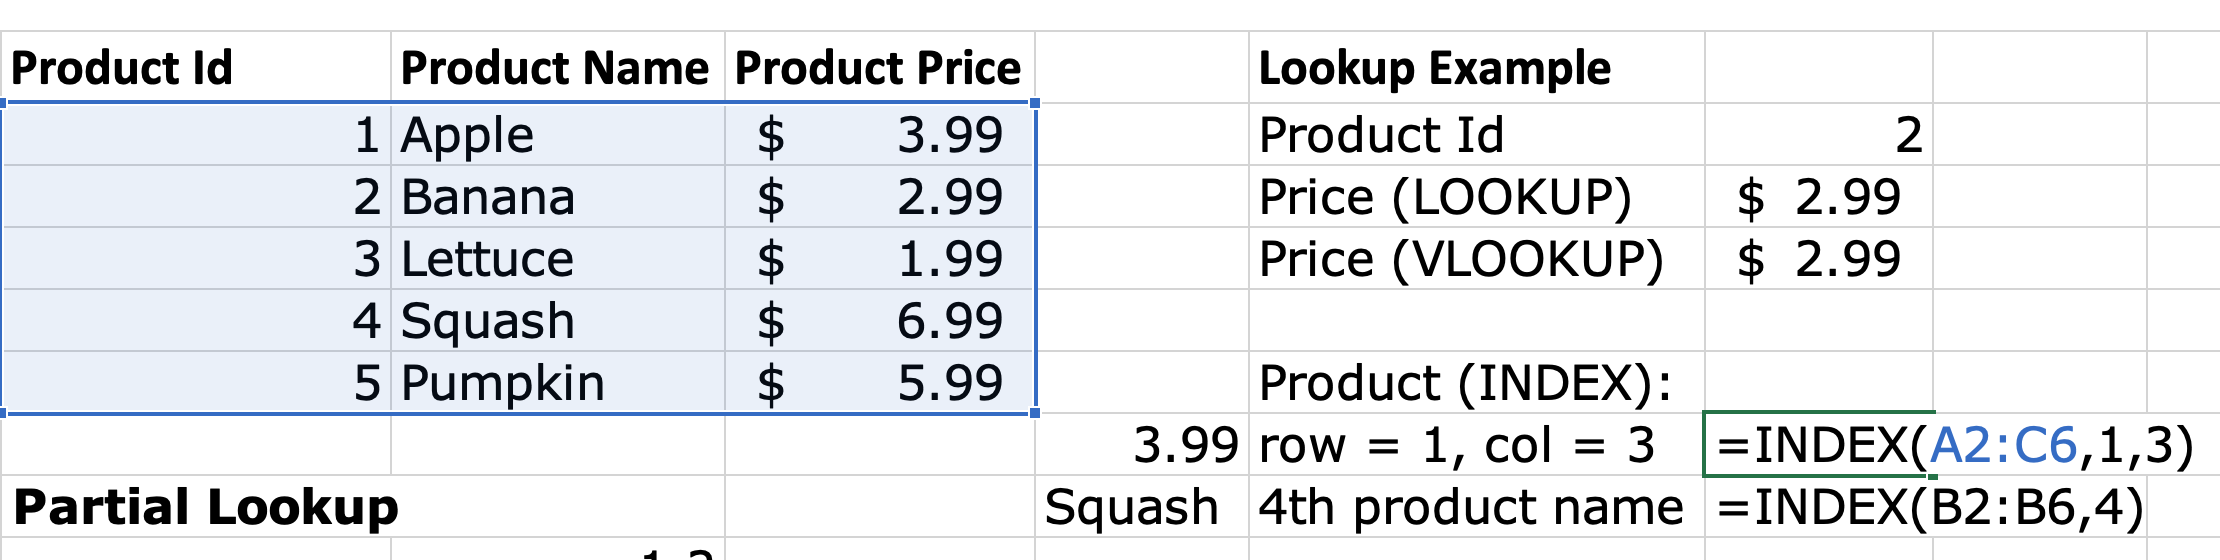
\includegraphics[width=0.9\textwidth]{img/indexZoom}
\end{center}
\end{frame}






\begin{frame}{Formulas Question}
\begin{example}
How many of the following statements are TRUE?
\begin{enumerate}
\item {\tt CONCATENATE} function can take 3 arguments.
\item There is an Excel function that has 0 arguments.
\item \texttt{=INDEX(\{1,3,5\},2)} returns 5.
\item {\tt =LOOKUP(5,\{1,3,5\},\{"a","b","c"\})} returns {\tt "c"}.
\end{enumerate}
\begin{enumerate}[A)]
\item  0		
\item 1		
\item 2		
\item 3		
\end{enumerate}
\end{example}
\end{frame}



\begin{frame}<handout:0>[fragile]{Formulas Question}
\begin{block}
{Answer:} How many of the following statements are TRUE?
\begin{enumerate}
\item {\color<1->{ForestGreen}{\texttt{CONCATENATE} function can take 3 arguments.}}
\item {\color<2->{ForestGreen}{There is an Excel function that has 0 arguments.} eg. {\tt NOW()}}
\item {\color<3->{red}{\texttt{=INDEX(\{1,3,5\},2)} returns 5.}}
\item {\color<4->{ForestGreen}{\texttt{=LOOKUP(5,\{1,3,5\},\{"a","b","c"\})} returns {\tt "c"}.}}
\end{enumerate}
\begin{enumerate}[A)]
\item  0		
\item 1		
\item 2		
\item \textbf<4>{\textit<4>{{\color<4>{iyellow}{3}}}}
\end{enumerate}
\end{block}
\end{frame}


\begin{frame}[fragile]{Advanced Spreadsheet Addressing}
The dollar sign ``\blue{\tt\$}'' is a symbol that indicates an \emph{absolute address}.  
\begin{itemize}
\item By default, addresses are "relative" in the sense that if they are in a formula that is copied to another cell, they will be changed relative to where they were copied from their origin.
\end{itemize}
Example:
\begin{itemize}
\item Cell \cell{A1} has the formula {\tt =A2+B1}
\item Copy contents of cell \cell{A1} to cell \cell{C4} (+ 2 columns + 3 rows).  
\item Formula changes to {\tt =C5+D4} because moved down three rows and over two columns. (eg. col\cell{A} + 2col = \cell{C}, row\cell{2} + 3 = 5; hence \cell{A2} changes to \cell{C5})
\end{itemize}
If cell \cell{A1} had the formula \verb|=$A$2+$B$1|, then the same formula would be copied in cell \cell{C4}.
\end{frame}

%\begin{frame}[fragile]{Advanced Spreadsheet Addressing}
%You can three different ways you can specify an absolute address
%\begin{itemize}
%\item By row eg. \verb|=B$1|
%\item By column eg. \verb|=$B1|
%\item By cell (row and column) eg. \verb|=$B$1|
%\end{itemize}
%  \begin{exampleblock}{}
%Question: How would the formula \verb|=$A2+B$3| in cell \cell{D3} be changed when copied to \cell{E5}?  \end{exampleblock}
%\end{frame}


\begin{frame}[fragile]{Advanced Spreadsheet Addressing}
There are three different ways you can specify an absolute address
\begin{itemize}
\item By row eg. \verb|=B$1| (column will change but row will not)
\item By column eg. \verb|=$B1| (row will change but col will not)
\item By cell (row and column) eg. \verb|=$B$1| (neither row nor col will change)
\end{itemize}
  \begin{exampleblock}{}
Question: How would the formula \verb|=$A2+B$3| in cell \cell{D3} be changed when copied to \cell{E5}?  \end{exampleblock}
\only<beamer:2-|handout:0>{\cell{D3} to \cell{E5}:  $\rightarrow$ one column, $\downarrow$ two rows\\}
\begin{itemize}
\item<beamer:3-|handout:0>{\verb|$A2|:  + \st{$\rightarrow$ one column}, $\downarrow$ two rows = \verb|$A4|\\}
\item<beamer:4-|handout:0> {\verb|B$3|:  + {$\rightarrow$ one column}, + \st{$\downarrow$ two rows} = \verb|C$3|\\}
\end{itemize}
\begin{block}<beamer:5-|handout:0> 
{}Answer: The copied formula would appear as \verb|=$A4+C$3| in cell \cell{E5}
\end{block}
\end{frame}

\begin{frame}{Formulas and Reference Question}
\begin{example}{}
 Cell \cell{A1} contains the following: =\$B2+D\$4. What is the formula if the cell is copied to cell D3?
\begin{itemize}
\item error
\item =\$B2+D\$4
\item =\$B4+F\$4
\item =\$B4+G\$4
\end{itemize}
\end{example}
For more examples see the {\bf Absolute} worksheet on  {\sf DemoPartI} 
\end{frame}

\begin{frame}<handout:0>{Formulas and Reference Answer}
\begin{block}{Answer:}
 Cell A1 contains the following: =\$B2+D\$4. What is the formula if the cell is copied to cell D3?
\begin{itemize}
\item error
\item =\$B2+D\$4
\item =\$B4+F\$4
\item \answer{=\$B4+G\$4}
\end{itemize}
\end{block}
\end{frame}


\begin{frame}{Tips}
\begin{alertblock}
{\bf Tip:} You can change a cell from relative to absolute with the shortcut  \keystroke{F4}. You can continue to press F4 to have Excel cycle through the different reference types.
\end{alertblock}
\begin{alertblock}
{\bf Tip:} To show all the formulas in  a worksheet (rather then their result), click the 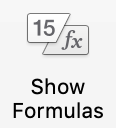
\includegraphics[height=2em]{showFormula} \ button located in the {\bf Formulas} tab in the ribbon.
\end{alertblock}

\end{frame}





\begin{frame} {Naming Cells}
Instead of referring to cells by their address, you can give a cell
a name and use that name in cell formulas.
\begin{itemize}
\item This makes it easier to read and understand formulas.
\item Like programming variables where we use names instead of addresses
to refer to data locations.
\end{itemize}
%Click the letter of the column you want to change and then click the ``Formulas'' tab. Click ``Define Name'' in the Defined Names group in the Ribbon to open the New Name window.
%\begin{center}
%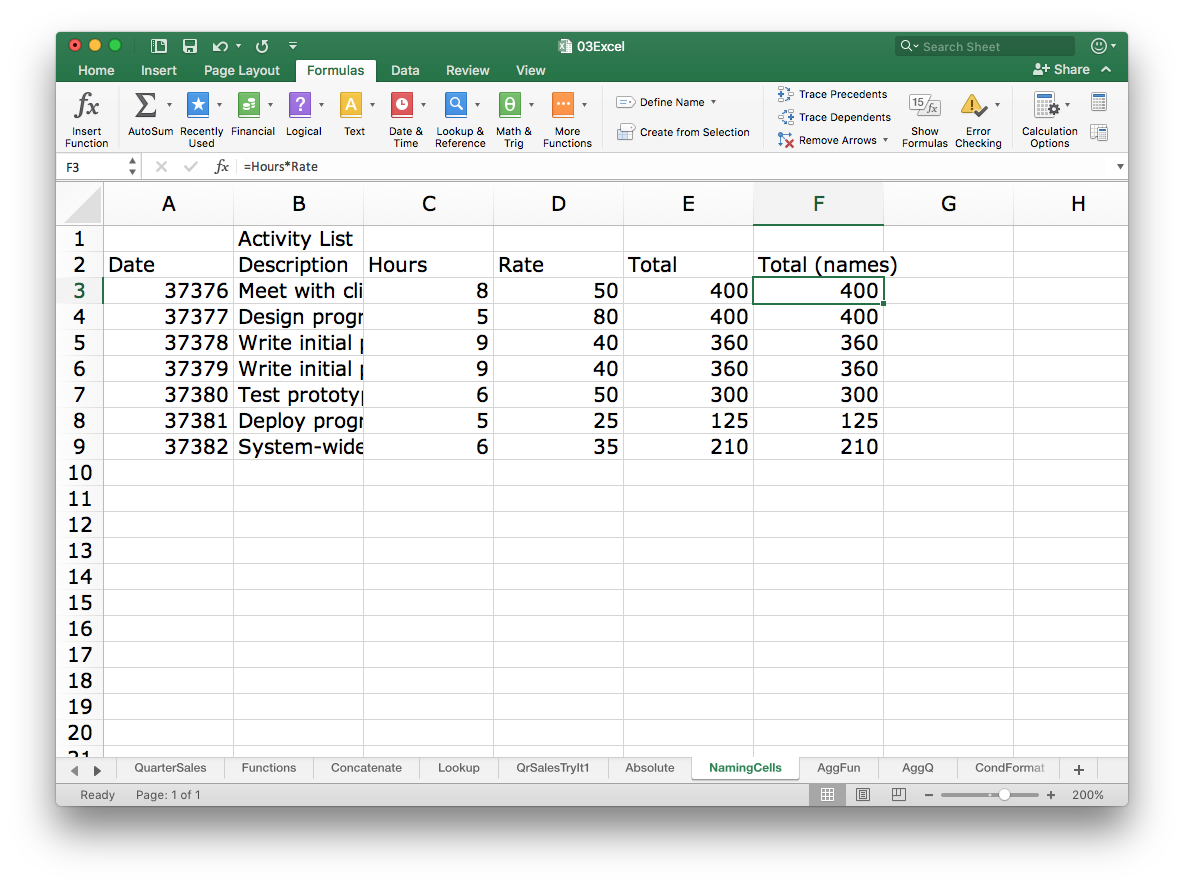
\includegraphics[width=0.8\textwidth]{img/DefineNames.png}
%\end{center}
\end{frame}


\begin{frame} {Naming Cells}
Step for naming cells:
 \begin{itemize}
\item Select the cell(s) you want to name
\item Click the Name box located to the left of the formula bar
\item Type a valid one-word name for the list, e.g. Hours
\item Press \keystroke{ENTER} \hfill \href{https://youtu.be/eEFbCBCLLFM}{See YouTube demo here}
\end{itemize}
Alternatively: click the letter of the column you want to change and then click the ``Formulas'' tab. Click ``Define Name'' in the Defined Names group in the Ribbon to open the New Name window.
\begin{center}
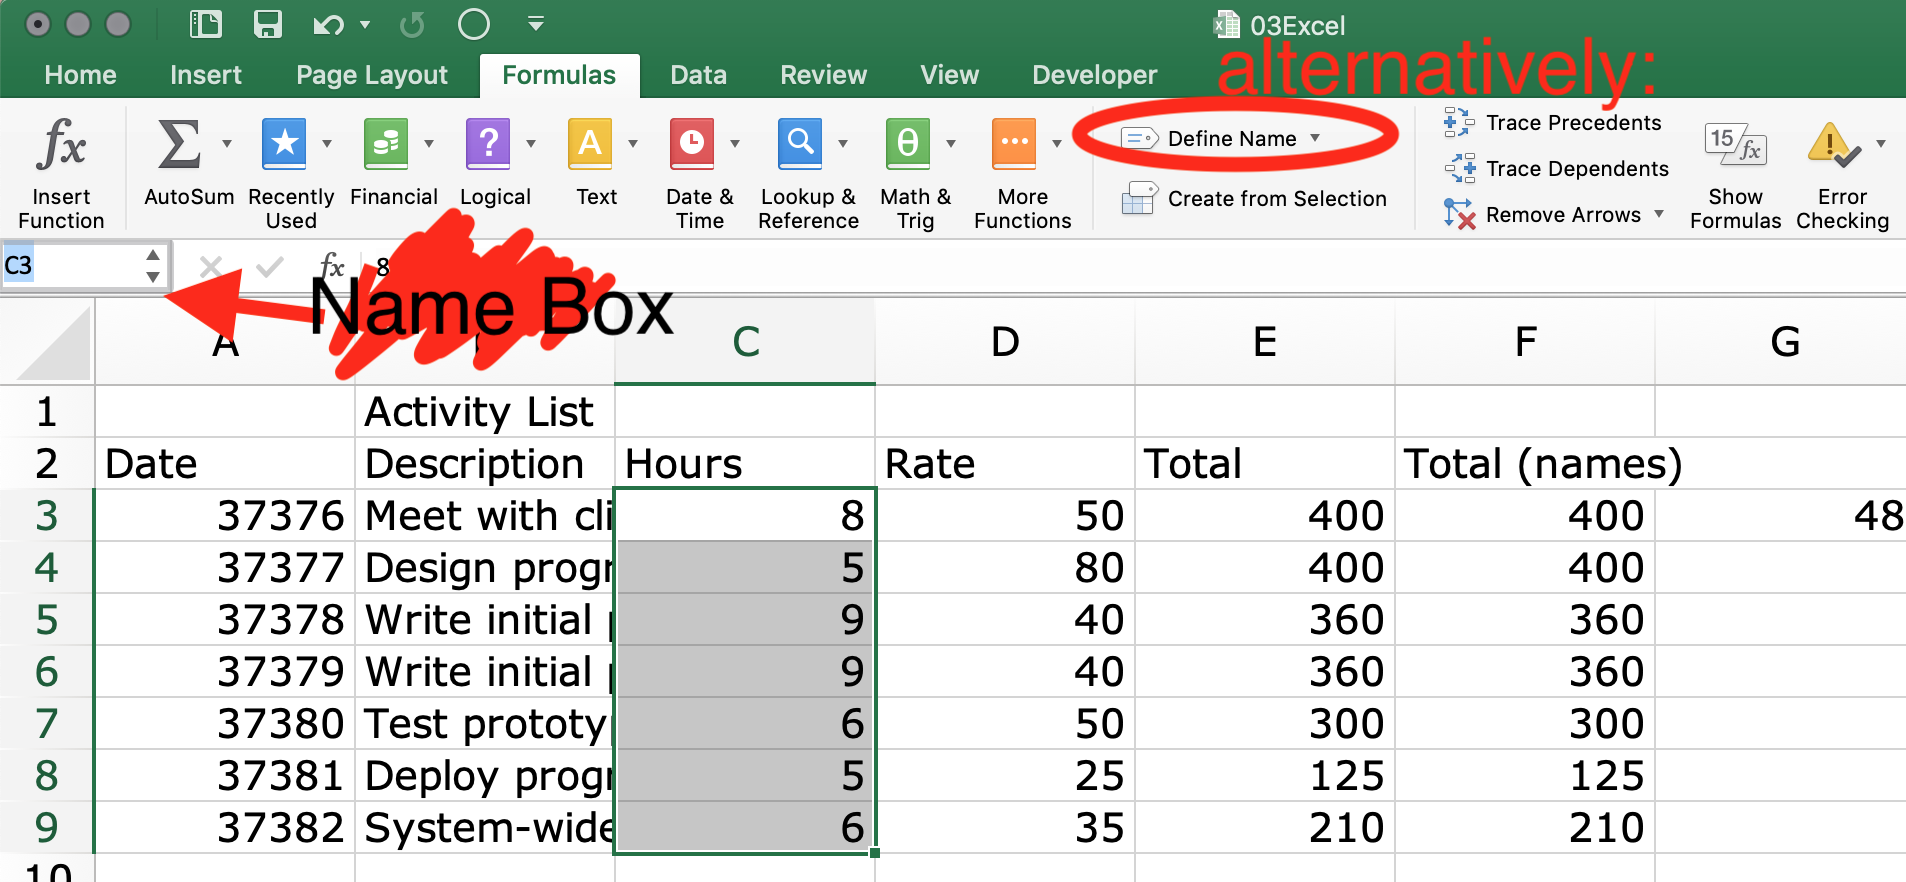
\includegraphics[width=0.8\textwidth]{img/NameBox}
\end{center}
\end{frame}

\begin{frame}{Naming Rules}
\begin{itemize}
\item While these names can included numbers, the first character must be a letter or an underscore. 
\medskip
\item These names cannot include spaces or special characters beside underscores and periods.  
\medskip
\item Finally this name should not conflict with an existing name in the workbook.
\medskip
\item For example, I wouldn't want to use the name {\tt DAY1} since that already exists as a cell address by default.
\end{itemize}
\end{frame}

\begin{frame}{Try It!}
Complete the following in the \textit{NamedCells} worksheet in the {\sf DemoPartI} workbook.
\begin{example}
Rename \cell{A3} \textit{Day\_1} and \cell{A9} \textit{Day\_7}.  Calculate the difference between these two dates using the \href{https://exceljet.net/excel-functions/excel-datedif-function}{DATEDIF} function.
\end{example}
\begin{example}
Find the total hours using named cells.  That is, rename the cells \cell{E3}:\cell{E9} \textit{Total} and calculate {\tt =SUM(Total)}. 
\end{example}

\begin{example}[Advanced array formulas]
Recalculate the Totals using the named cells.  That is, rename the cells \cell{C3}:\cell{C9} \textit{Hours} and \cell{D3}:\cell{D9} \textit{Rate}, and calculate {\tt Hours*Rate}. 
\end{example}
To answer this last exercise, we will need to know more about \hyperlink{arrayfun}{array formulas}.
\end{frame}


\begin{frame}{Array Formulas}\label{arrayfun}
\begin{itemize}
\item If you are using Office 2010 -- Office 2019 array formulas require first selecting the entire output range, then confirming the formula with \keystroke{Ctrl}+\keystroke{Shift}+\keystroke{Enter}. They are commonly referred to as CSE formulas.
\medskip
\item In Office 365 any formula that can return multiple results will automatically spill them either down, or across into neighboring cells by pressing \keystroke{Enter}.
\medskip
\item To see Total cost of each activity, select cells \cell{F3}:\cell{F9}, enter the formula {\tt =Hours*Rate}, and then press \keystroke{Ctrl}+\keystroke{Shift}+\keystroke{Enter}.
\medskip
\item N.B. To see the grand Total of all activities, we could select cell \cell{F10} and enter the formula {\tt =SUM(Hours*Rate)} and then press \keystroke{Ctrl}+\keystroke{Shift}+\keystroke{Enter}.
\end{itemize}
 Read more about array formulas \href{https://support.office.com/en-ie/article/guidelines-and-examples-of-array-formulas-7d94a64e-3ff3-4686-9372-ecfd5caa57c7}{here}. See my YouTube demo \href{https://youtu.be/rHqKVJJmuFs}{here}.
\end{frame}


\begin{frame}[fragile]{Aggregate Functions}
An \emph{aggregate} function computes a summary function over a range of cells.  The values can either be data values or cell locations. 
Common functions are:
\begin{center}
\begin{tabular}{|l|l|}
\hline
{\tt =MIN(<value list>)} 	& returns minimum value in list \\ \hline
{\tt =MAX(<value list>)}	& returns maximum value in list\\\hline
{\tt =SUM(<value list>)}	& returns sum of all values in list\\\hline
{\tt =AVERAGE(<value list>)} 	& returns average of values in list\\\hline
{\tt =COUNT(<value list>)} 	& returns count of values in list\\\hline
{\tt =MEDIAN(<value list>)} 	& returns median value of list \\\hline
\end{tabular}
\end{center}
If specifying an array, give the upper left and lower right corners, separated by a colon.
\begin{center}
\begin{tabular}{|l|p{6cm}|}
\hline
 {\tt AVERAGE(A3:E6)}  & returns the average value in the array of 4 rows and 5 columns\\\hline
\end{tabular}
\end{center}
\end{frame}

\begin{frame}{Aggregate Functions Example}
\hspace*{-6mm}                                                           
 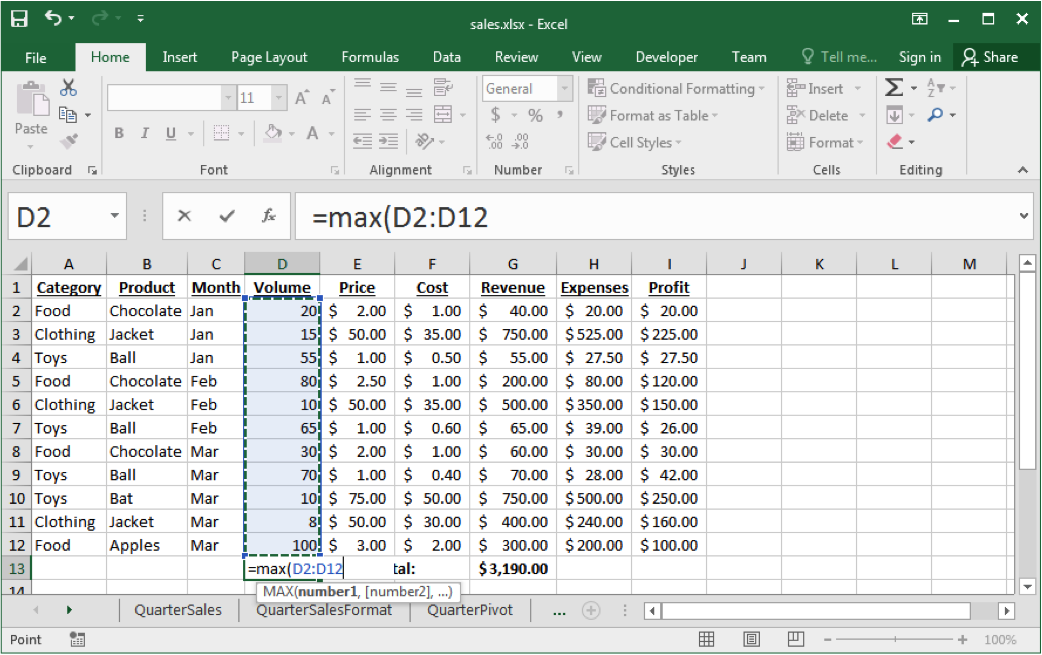
\includegraphics[width=1.1\textwidth]{aggregate}
\end{frame}



\begin{frame}{Try it!}
\begin{exampleblock}{Exercise}
Find the a) maximum volume b) average price c) minimum cost and d) total revenue in the \textit{QrSales} worksheet.
\end{exampleblock}
\end{frame}


\begin{frame}{Aggregate Functions Question}
  \begin{example}
Assume the cells in the range {\tt A1:C4} each contain a number that is equal to their row number (e.g. \cell{B3} contains {\tt 3}). How many of the following statements are TRUE?
\begin{enumerate}
\item The number of cells in the range is 12.
\item The value of {\tt SUM(A1:C4)} is 20.
\item The value of {\tt COUNTIF(A1:B4,">2")} is 4.
\item {\tt AVERAGE(A1:C4) > MAX(C2:C3)}
\end{enumerate}
\begin{multicols}{5}
\begin{enumerate}[A)]
\item 0 
\item 1
\item 2
\item 3
\item 4
\end{enumerate}
\end{multicols}
  \end{example} 
\end{frame}





\begin{frame}<handout:0>{Aggregate Functions Question}
  \begin{block}{Answer:}
Assume the cells in the range {\tt A1:C4} each contain a number that is equal to their row number (e.g. \blue{B3} contains {\tt 3}). How many of the following statements are TRUE?
\begin{enumerate}
\item {\color<2->{sgreen}{The number of cells in the range is 12.}}
\item {\color<3->{red}{The value of {\tt SUM(A1:C4)} is 20... should be 30}.}
\item {\color<4->{sgreen}{The value of {\tt COUNTIF(A1:B4,">2")} is 4}.}
\item {\color<5->{red}{\tt AVERAGE(A1:C4) > MAX(C2:C3)}} 
\end{enumerate}
\begin{multicols}{5}
\begin{enumerate}[A)]
\item 0 
\item 1
\item \textbf<6>{\textit<6>{{\color<6>{iyellow}{2}}}}
\item 3
\item 4
\end{enumerate}
\end{multicols}
  \end{block} 
\end{frame}




\begin{frame}{Aggregate Functions Question}
  \begin{example}
Assume the three cells in the range A1:C1 contain numbers.  Which of these formula output results is ALWAYS the largest?
\begin{enumerate}[A)]
\item {\tt MAX(A1:C1)}
\item {\tt MIN(A1:C1)}
\item {\tt COUNT(A1:C1)}
\item {\tt SUM(A1:C1)}
\item {None of the above are always guaranteed to be the largest}
\end{enumerate}
 \end{example} 
\end{frame}



\begin{frame}<handout:0>{Aggregate Functions Question}
  \begin{block}{Answer:}
Assume the three cells in the range A1:C1 contain numbers.  Which of these formula output results is ALWAYS the largest?
\begin{enumerate}[A)]
\item {\tt MAX(A1:C1)}
\item {\tt MIN(A1:C1)}
\item {\tt COUNT(A1:C1)}
\item {\tt SUM(A1:C1)}
\item \answer{None of the above are always guaranteed to be the largest}
\end{enumerate}
 \end{block} 
\end{frame}



\begin{frame}{Other Formatting: Column Width}
 {Resizing columns/rows:}
\begin{columns}[T] % align columns
\begin{column}{.65\textwidth}
 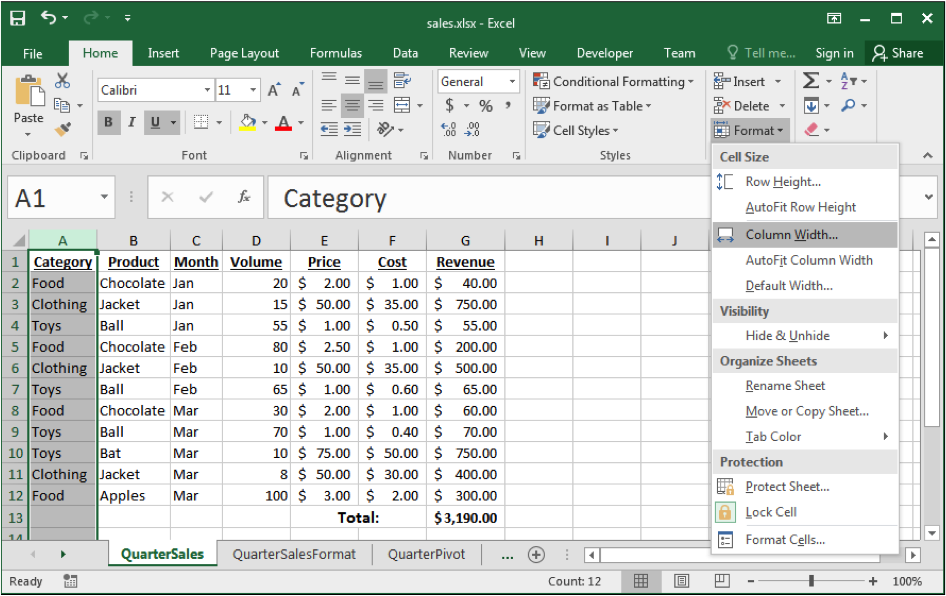
\includegraphics[width=1.1\textwidth]{ColWidth.png}
\end{column}%
\hfill%
\begin{column}{.33\textwidth}
{\color{blue}\rule{\linewidth}{4pt}}
Auto-resize by double clicking on border between columns or selecting \textbf{Format}-->\textbf{Column}-->\textbf{AutoFit Selection}.\\[1em]
Drag the row/column border to manually resize.
{\color{blue}\rule{\linewidth}{4pt}}
\end{column}%
\end{columns}
Lets see an example by doing this on the \textit{Namecells} workbook in DemoPartI
\end{frame}

% https://support.office.com/en-us/article/use-data-bars-color-scales-and-icon-sets-to-highlight-data-f118d0a6-5921-4e2e-905b-fe00f3378fb9
\begin{frame}{Conditional Formatting}
\emph{Conditional formatting} allows you to change the cell format based on data values.  This is accessible under \textbf{Format}-->{\bf Conditional Formatting}.
\begin{itemize}
\item Other options: data bars, color scales, icon sets
\end{itemize}
\hspace*{-6mm}         
\begin{center}                                                  
 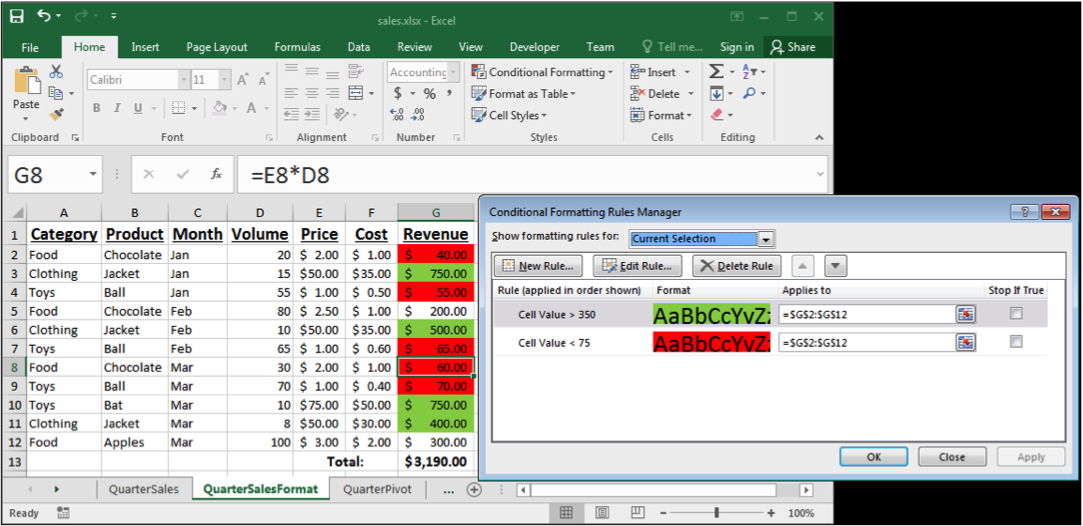
\includegraphics[width=.8\textwidth]{CondFormat}
 \end{center}
\end{frame}



\begin{frame}{Conditional Formatting}
A shortcut to this feature (along with some great default options) can be found in the Conditional Formatting button  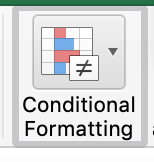
\includegraphics[width=3em]{CFbutton}.

\begin{center}
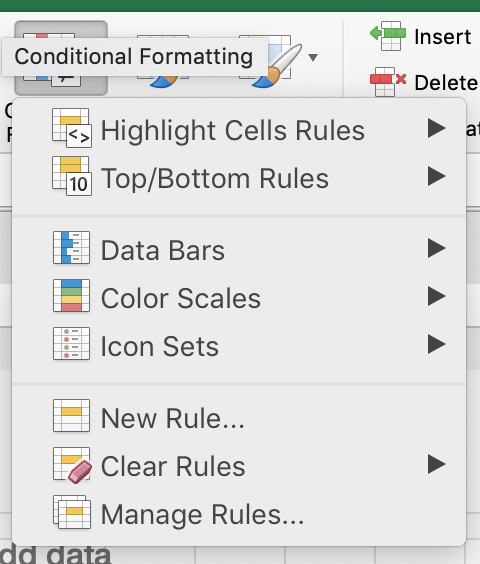
\includegraphics[height=0.4\textheight]{CFoptions}
\end{center}


\end{frame}

\begin{frame}{Conditional Formatting Result}
The format painter button allows you to copy formatting to many cells.  Select the cell, click paint button, then highlight cells to have identical formatting.
\hspace*{-6mm}                                                           
 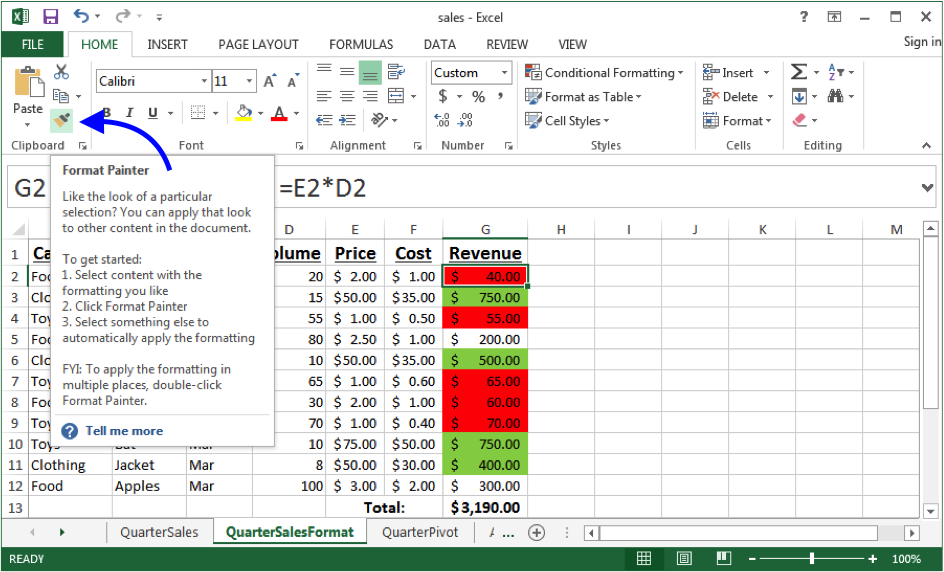
\includegraphics[width=1.1\textwidth]{FormatPainter}
\end{frame}

\begin{frame}{Try it: Conditional Formatting}
  \begin{exampleblock}{}{Format Volume column to be:}
\begin{enumerate}
\item bold/green if volume $> 50$
\item italics/red if volume $< 10$
\item yellow background otherwise as below:
\end{enumerate}
  \end{exampleblock}
\begin{center}
 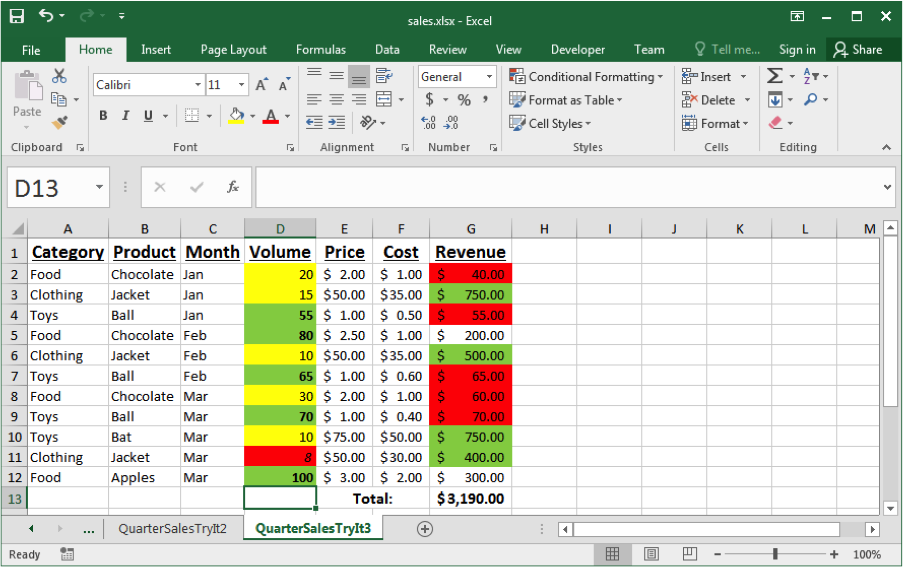
\includegraphics[width=.8\textwidth]{CondFormatTryIt}
\end{center}
\end{frame}


\begin{frame}{Try it: Conditional Formatting}
  \begin{exampleblock}{Question:}
Take the previous formatting and apply it to whole row:
  \end{exampleblock}
  Hint: Highlight the whole table, go to Conditional Formatting, select the ``Classic" option from the Style drop down menu and select ``Use a formula to determine which cells to format"
\begin{center}
 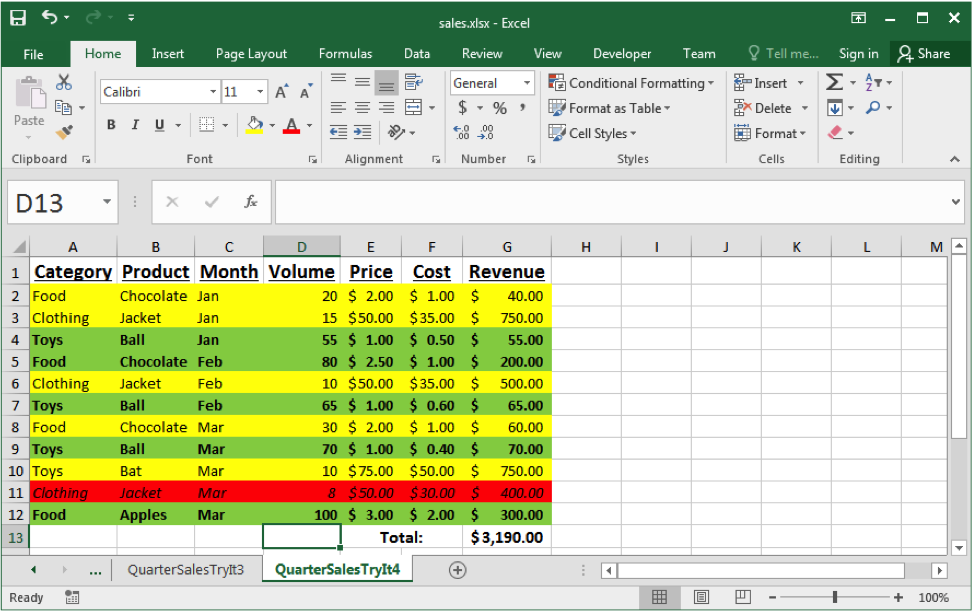
\includegraphics[width=.8\textwidth]{QSTryIt4}
\end{center}
\end{frame}


\begin{frame}<handout:0>
\begin{center}
 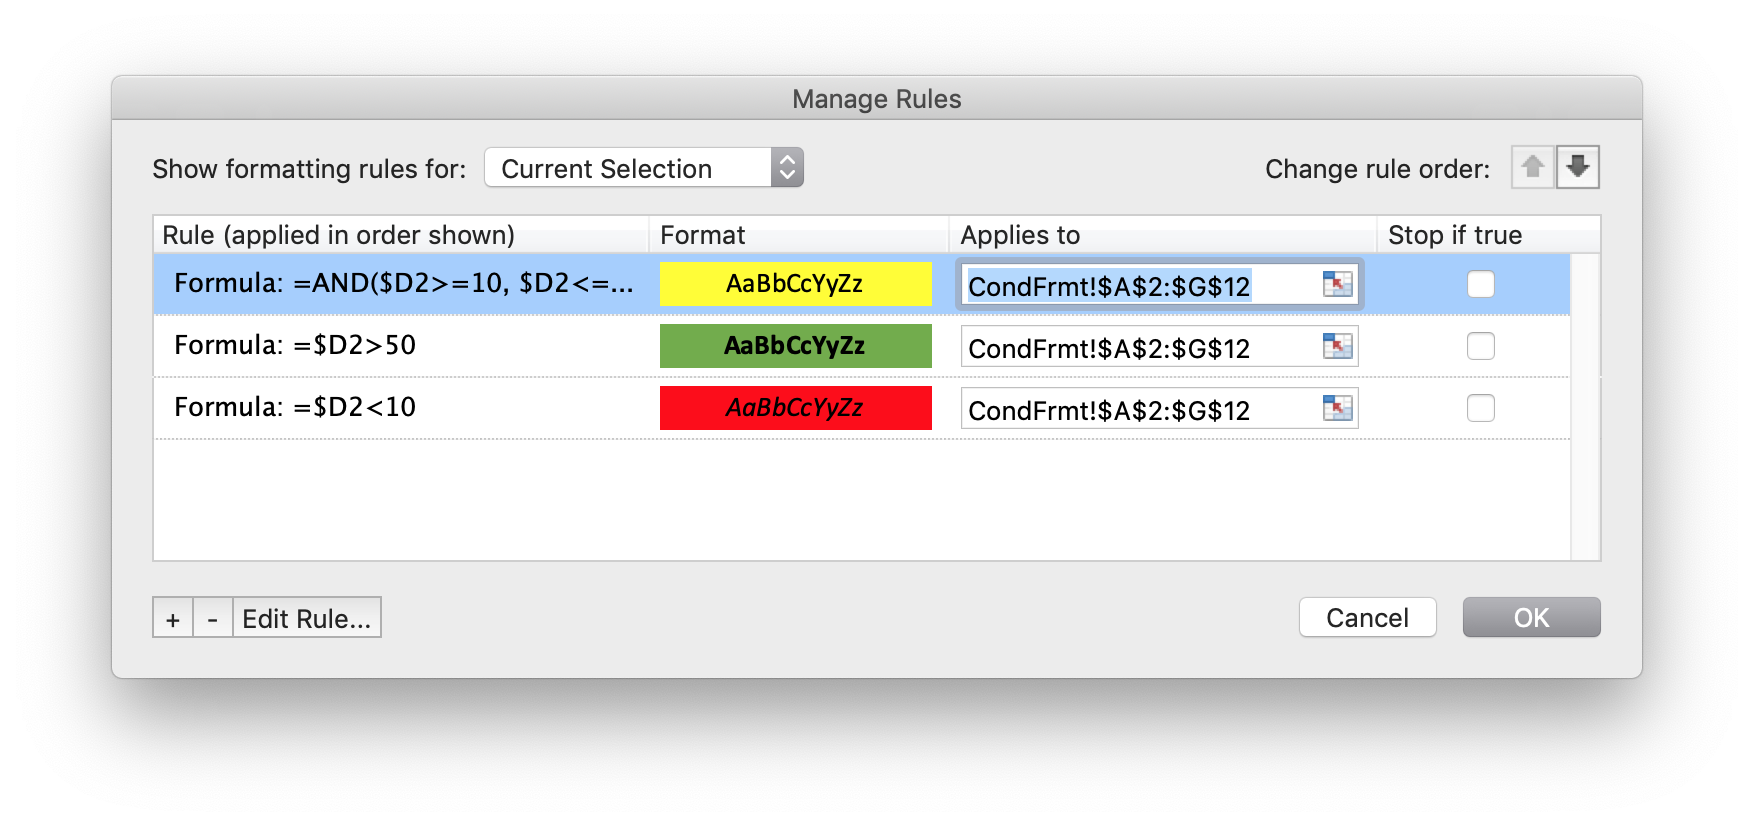
\includegraphics[width=.8\textwidth]{condform2}
\end{center}
\vspace{-1cm}
\begin{center}
 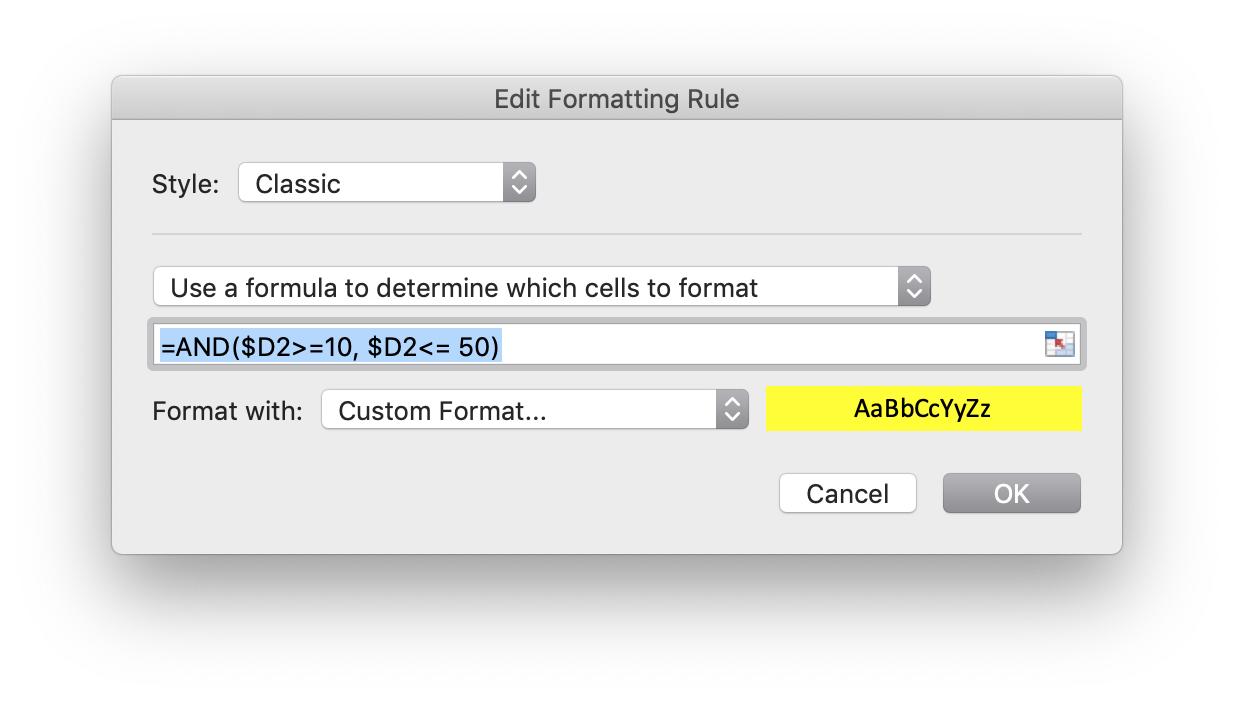
\includegraphics[width=.8\textwidth]{condform1}
\end{center}
\end{frame}




\begin{frame}{Spreadsheet for Data Management}
A spreadsheet is often used as a "database".  A \emph{database}  collects, stores and manages information
so users can retrieve, add, update or remove such
information.
\begin{itemize}
\item Examples: schedules and calendars, timesheets, expenses and finances, records, notes, and recipes, data research/analysis
\end{itemize}
We can use a spreadsheet as a database by:
\begin{itemize}
\item Using a row to store all the information about something we want to represent.
\item Giving each column a meaningful name.  A column represents a property or feature of the object stored in the row.
\item Using the formulas to calculate new facts from the data.
\item Using sorting to organize the data by key features.
\item Using simple filtering (querying) to only show the most important data or data of interest. 
\end{itemize}
\end{frame}
% https://www.webopedia.com/TERM/Q/query.html
%  A query is a request for information from a database. There are three general methods for posing queries:


\begin{frame}{Sorting Data}
Data can be sorted by selecting the {\bf Sort} option under the {\bf Data} menu.  Select the column(s) to sort on and order to sort by.
\begin{center}
 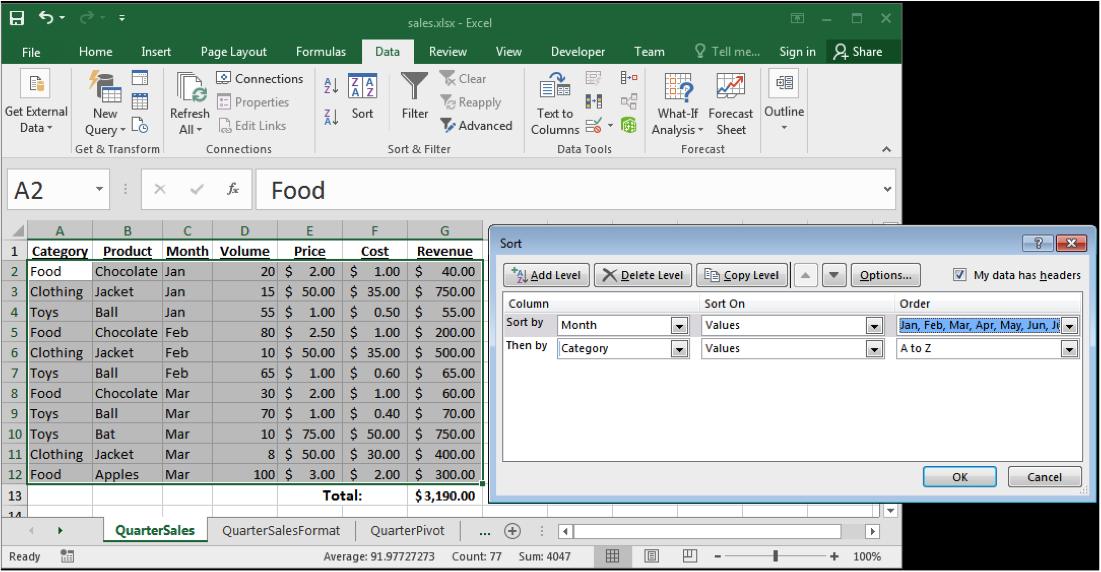
\includegraphics[width=.99\textwidth]{Sorting}
\end{center}
\end{frame}

\begin{frame}{Try it: Sorting Data}
  \begin{exampleblock}{}{}
{\bf Exercise}: Sort the data by revenue (desc) then product (asc).
  \end{exampleblock}
\begin{center}
 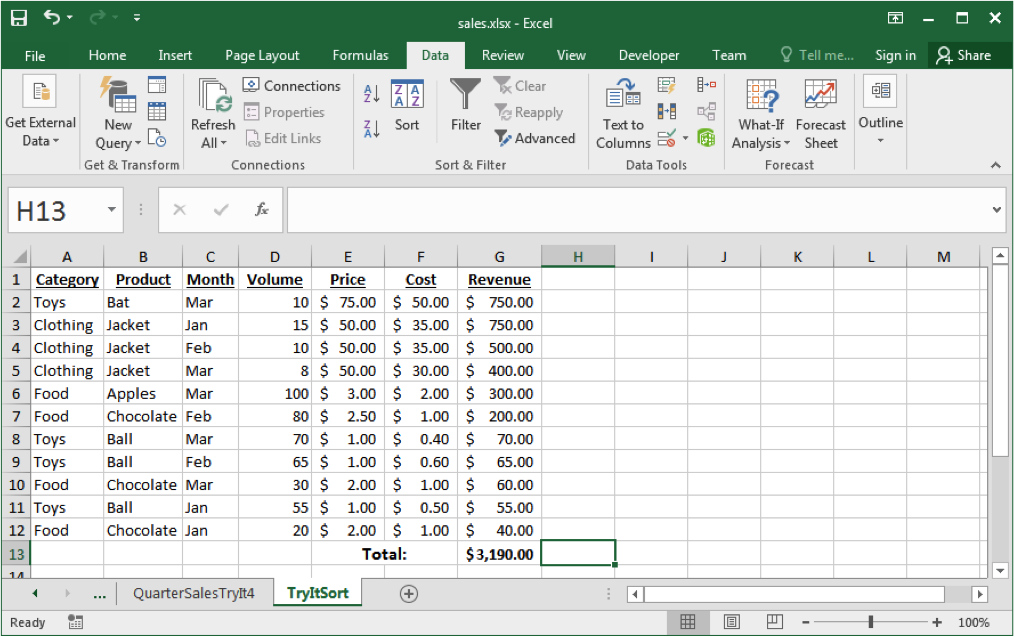
\includegraphics[width=.9\textwidth]{SortQ}
\end{center}
\end{frame}

\begin{frame}{Filtering}
A \emph{filter} shows a subset of the rows in the spreadsheet that pass a given condition (test).\\[1em] 
Select {\bf Auto Filter} under the {\bf Data} then {\bf Filter} menu.\\[1em] 
Once you select {\bf Auto Filter}, each column heading has a drop-down list.  By selecting a filtering criteria from the list, you can limit the rows that are displayed.\\[1em] 
It is possible to filter on more than one column at the same time.
\end{frame}



\begin{frame}{Filter Example}
Filter on Revenue column:  Select value(s), Top 10, or custom filter.
\begin{center}
% 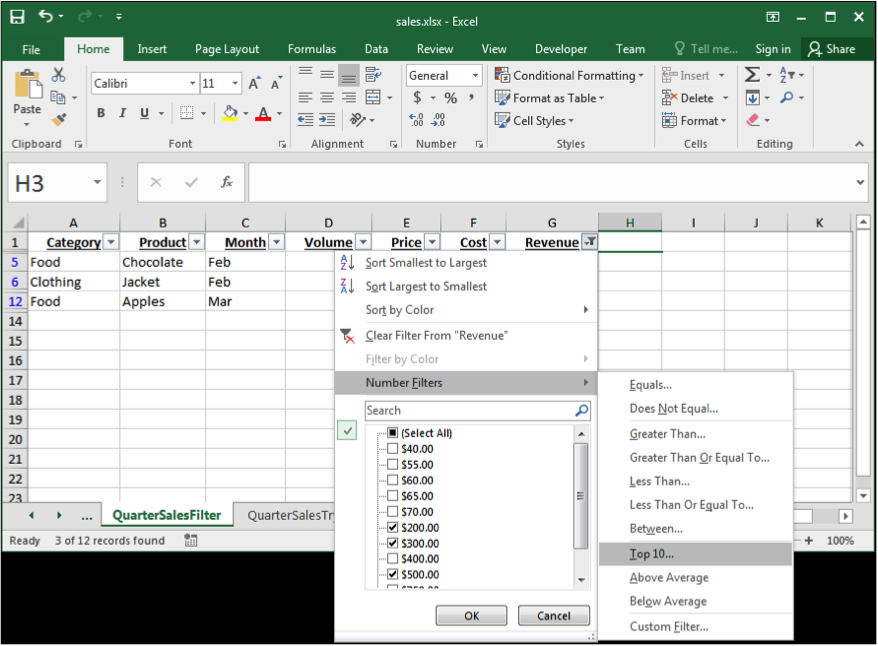
\includegraphics[width=.8\textwidth]{FilterEg}
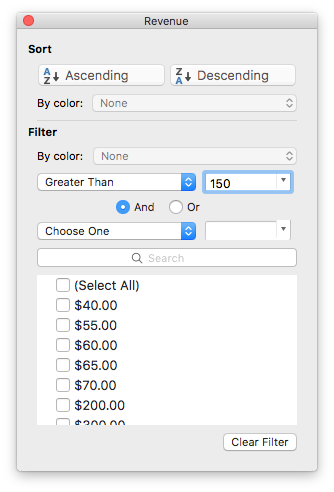
\includegraphics[width=.5\textwidth]{CustomFilter}
\end{center}
\end{frame}


\begin{frame}{Filter Example}
Filter on Revenue column:  Custom filter with Revenue > 150
\begin{center}
 \includegraphics[width=.8\textwidth]{CustomFilter2}
% \includegraphics[width=.8\textwidth]{GT150}
\end{center}
\end{frame}


%\begin{frame}{Filter Example}
%Filter on Revenue:  Custom filter result with Revenue > 150
%\begin{center}
% \includegraphics[width=.99\textwidth]{GT150out}
%\end{center}
%\end{frame}
%
%\begin{frame}{Try It: Filter Example}
%Question: Filter the data so only products with volume < 50 and revenue < \$100 are shown.
%\begin{center}
% \includegraphics[width=.99\textwidth]{GT150out}
%\end{center}
%\end{frame}


\begin{frame}{Try It: Filter Challenge}
\begin{exampleblock}{}
{\bf Exercise}: Filter the data so only products with volume < 20 or revenue $\geq$ \$500 are shown.\end{exampleblock}


\begin{center}
 \includegraphics[width=.99\textwidth]{FilterChallenge}
\end{center}
\end{frame}


\begin{frame}[fragile]{Removing Duplicates}


To remove duplicates, select your Data then {\bf Remove Duplicates} from the {\bf Data} tab in the ribbon.
\begin{center}
 \includegraphics[width=.7\textwidth]{RmDup}
\end{center}

Note that we can also remove duplicates using a filter:
$$Data > Sort \& Filter > Advanced$$

\begin{minipage}{0.6\textwidth}\raggedleft
By default, it will look for duplicates over the all of the selected columns.  You can delete entire rows based on particular columns by selecting them the pop-up window:
\end{minipage}
\hfill
\noindent\begin{minipage}{0.3\textwidth}% adapt widths of minipages to your needs
\includegraphics[width=\linewidth]{removedup}
\end{minipage}%

\end{frame}


\begin{frame}{Removing Duplicates}


Notice how the Removing Duplicates feature is NOT case sensitive:
\begin{center}
 \includegraphics[width=.7\textwidth]{rmDup2}
\end{center}



\end{frame}



\begin{frame}{Sorting Question}
\begin{exampleblock}{Question:} Given this spreadsheet and sort order, what is the output?
\end{exampleblock}
\begin{columns}[T] % align columns
\begin{column}{.65\textwidth}
\vspace{5em}
  \includegraphics[width=1.15\textwidth]{SortingQ2}
\end{column}%
\hfill%
\begin{column}{.33\textwidth}
  \includegraphics[height=0.7\textheight]{SortingQuestion}
  \end{column}%
\end{columns}
\end{frame}


\begin{frame}{Sorting Question}
\begin{exampleblock}{Clicker Question:} Given this spreadsheet and sort order, what is the output?
\end{exampleblock}
\begin{columns}[T] % align columns
\begin{column}{.33\textwidth}
\vspace{-1em}
\begin{enumerate}[A)]
% A is ordering by ASCII character value (asc).
\item 
\item[]
\end{enumerate}
\vspace{-1em}
 \includegraphics[height=.6\textheight]{sortA}
\end{column}%
\hfill%
\begin{column}{.33\textwidth}
\vspace{-1em}
\begin{enumerate}[B)]
\item 
\end{enumerate}
    \includegraphics[height=.6\textheight]{sortB}
  \end{column}%
\begin{column}{.33\textwidth}
\vspace{-1em}
\begin{enumerate}[C)]
\item 
\end{enumerate}
      \includegraphics[height=.6\textheight]{sortC}
\end{column}%
\hfill%
\end{columns}
\end{frame}


\begin{frame}<handout:0>{Sorting Question}
\begin{exampleblock}{Question:} Given this spreadsheet and sort order, what is the output?
\end{exampleblock}
\begin{columns}[T] % align columns
\begin{column}{.33\textwidth}
\vspace{-1em}
\begin{enumerate}[A)]
% A is ordering by ASCII character value (asc).
\item \red{Wrong:}{\color<2->{red}{ Char desc from Z to A}}
\end{enumerate}
 \includegraphics[height=.6\textheight]{sortA}
\end{column}%
\hfill%
\begin{column}{.33\textwidth}
\vspace{-1em}
\begin{enumerate}[B)]
\item {\color<3->{red}{Wrong: case-sensitive}}
\end{enumerate}
    \includegraphics[height=.6\textheight]{sortB}
  \end{column}%
\begin{column}{.33\textwidth}
\vspace{-1em}
\begin{enumerate}[C)]
\item {\color<4>{sgreen}{Correct: default is not case-sensitive}}
\end{enumerate}
      \includegraphics[height=.6\textheight]{sortC}
\end{column}%
\hfill%
\end{columns}
\end{frame}

\begin{frame}{Sorting}
If you want to make sorting on characters case sensitive, we need to select that in Options:
 \begin{center}
\includegraphics[width=0.9\textwidth]{img/caseSensitive.png}
 \end{center}
\end{frame}



\begin{frame}{Filtering Question}

% ADVANCED FILTERING TECHNIQUES! (not easy to do)
% https://www.ablebits.com/office-addins-blog/2016/09/07/excel-advanced-filter/#advanced-filter 
  \begin{example}
 Given this spreadsheet, how many of these statements are TRUE?
 \vspace{-7mm}
 \begin{center}
    \includegraphics[height=.4\textheight]{FilteringQ}
 \end{center}
 \vspace{-1em}
\begin{enumerate}
\item The data is sorted ascending by {\tt Number}.
\item Filter {\tt Number} > 3 shows 3 rows.
\item Filter {\tt Letter} >= "c" shows 3 rows.
\item Filter {\tt Number} < 3 OR \textbf{\tt Letter} > "b" shows 5 rows.
\end{enumerate}
\vspace{-5mm}
\begin{multicols}{5}
\begin{enumerate}[A)]
\item 0 
\item 1
\item 2
\item 3
\item 4
\end{enumerate}
\end{multicols}
  \end{example} 
\end{frame}


\begin{frame}<handout:0>{Filtering Question}
  \begin{block}{Answer:}
 Given this spreadsheet, how many of these statements are TRUE?
  \vspace{-7mm}
 \begin{center}
    \includegraphics[height=.4\textheight]{FilteringQ}
 \end{center}
 \vspace{-1em}
\begin{enumerate}
\item {\color<1->{sgreen}{The data is sorted ascending by {\tt Number}.}}
\item {\color<2->{red}{Filter {\tt Number} > 3 shows 3 rows.}}
\item {\color<3->{sgreen}{Filter {\tt Letter} >= "c" shows 3 rows.}}
\item {\color<4->{sgreen}{Filter {\tt Number} < 3 OR {\tt Letter} > "b" shows 5 rows.}}
\end{enumerate}
\vspace{-5mm}
\begin{multicols}{5}
\begin{enumerate}[A)]
\item 0 
\item 1
\item 2
\item \textbf<5>{\textit<5>{{\color<5>{iyellow}{3}}}}
\item 4
\end{enumerate}
\end{multicols}
  \end{block} 
\end{frame}

\begin{frame}<handout:0>{Filtering Question}
N.B. The solution to the previous question required some \href{https://www.ablebits.com/office-addins-blog/2016/09/07/excel-advanced-filter}{Advanced Filtering} options:
 \begin{center}
    \includegraphics[height=.5\textheight]{advancedFilter}
 \end{center}

\end{frame}



\begin{frame}[label=current]{Conclusion}
\emph{Spreadsheets} are general purpose tools for data analysis that consist of a table of cells which contain data and formulas.\\[1em]
Formulas contain data values, cell references, and functions.
\begin{itemize}
\item Aggregate functions summarize multiple data values into a single value.
\item Functions exist for statistics, string manipulation, lookup/indexing, and decisions.
\end{itemize}
\end{frame}

\begin{frame}{Objectives}
\begin{itemize}
\item Explain what a spreadsheet is.
\item Explain how cells are addressed in a spreadsheet.
\item List some of the ways to select cells in a spreadsheet.
\item Define and explain: formula, function, argument, concatenation
\item Use these functions: concatenate, lookup, index
\item Explain the difference between an absolute and relative address.
\item Explain how an aggregate function works.  List some examples.
\item Explain how to use conditional formatting.
%\item Explain how spreadsheets can be used as a database.  
\end{itemize}
\end{frame}



\end{document}

